\documentclass[a4paper,13pt]{report}
% \usepackage[utf8]{vietnam}
\usepackage{iftex}
\ifPDFTeX
  \usepackage[utf8]{inputenc}
\else
  % XeTeX/Tectonic: cần phông OTF có đủ chữ Việt; Latin Modern giữ nguyên diện mạo của template.
  \usepackage{fontspec}
  \setmainfont{lmroman12-regular.otf}[BoldFont=lmroman12-bold.otf,ItalicFont=lmroman12-italic.otf,BoldItalicFont=lmroman10-bolditalic.otf]
  \setsansfont{lmsans10-regular.otf}[BoldFont=lmsans10-bold.otf,ItalicFont=lmsans10-oblique.otf]
  \setmonofont{lmmono12-regular.otf}
\fi
\usepackage[vietnamese=nohyphenation]{hyphsubst}
\usepackage[vietnamese]{babel}
% \usepackage[utf8]{inputenc}
\usepackage{amsmath}
\usepackage{amsfonts}
\usepackage{amssymb}
\usepackage{subcaption}
\usepackage{graphicx}
% \usepackage{caption}
\usepackage[font=small]{caption}
\usepackage{booktabs}
\usepackage[unicode]{hyperref}
\hypersetup{hidelinks}  % không vẽ khung màu quanh liên kết và trích dẫn
\usepackage[left=3cm,right=2cm,top=2.5cm,bottom=3cm]{geometry}
\usepackage{titlesec} 
\usepackage{scrextend}
\usepackage{enumerate}
\usepackage{tikz}
\usepackage{float}
\usepackage{afterpage}
\usepackage{multirow}
\usepackage{sectsty}
\usepackage{tocloft,calc}
\usepackage{listings}
\usepackage{makecell}
\usepackage[sort&compress]{natbib}
\usetikzlibrary{calc}
\usepackage{algorithm}
\usepackage{algpseudocode} 
\usepackage{longtable}
\usepackage{multirow}
\usepackage{tabularx}
\usepackage{float}
\usepackage{pgfplots}
\pgfplotsset{compat=1.16}
\usepgfplotslibrary{groupplots}
\usetikzlibrary{arrows.meta,positioning,fit,backgrounds,shapes.geometric,decorations.pathreplacing}
% \usepackage[perpage]{footmisc}
\usepackage{perpage} %the perpage package
\MakePerPage{footnote} %the perpage package command
% \usepackage[ruled,vlined]{algorithm2e}
\PassOptionsToPackage{table}{xcolor}

\def\changemargin#1#2{\list{}{\rightmargin#2\leftmargin#1}\item[]}
\let\endchangemargin=\endlist 

\changefontsizes{13pt}
\bibliographystyle{unsrt}

\makeatletter
\def\l@figure{\@dottedtocline{1}{1em}{2.2em}}
\def\l@table{\@dottedtocline{1}{1em}{2.2em}}
\renewcommand*{\ALG@name}{Thuật toán}
\makeatother

\sectionfont{\fontsize{15}{15}\selectfont}
\subsectionfont{\fontsize{13}{15}\selectfont}

\titleformat{\chapter}[display]   
{\normalfont\huge\bfseries}{\chaptertitlename\ \thechapter}{0pt}{\LARGE}
\titlespacing*{\chapter}{0cm}{-\topskip}{0pt}[0pt]

\renewcommand{\baselinestretch}{1.3}
%\renewcommand{\cftsecpresnum}{Chương\space}
\renewcommand{\cftchappresnum}{Chương }
% số mục hai chữ số (2.10, 2.11) cần chỗ rộng hơn
\setlength{\cftsecindent}{1em}
\setlength{\cftsecnumwidth}{3em}
\setlength{\cftsubsecindent}{4em}
\setlength{\cftsubsecnumwidth}{3.8em}
\AtBeginDocument{\addtolength\cftchapnumwidth{\widthof{\bfseries Chương }}}
\setlength{\parskip}{0.4em}
\setlength{\parindent}{0pt}
%
% Thông tin trình bày trên bìa và các trang đầu. Sửa tại đây, không sửa trong cover.tex.
\newcommand{\tensinhvien}{Dương Minh Vương}
\newcommand{\tendetai}{NGHIÊN CỨU, THIẾT KẾ VÀ PHÁT TRIỂN HỆ THỐNG GIA SƯ AI CÓ KHẢ NĂNG KIỂM CHỨNG BÁM SÁT CHƯƠNG TRÌNH HỌC TRÊN NỀN TẢNG WEB SỬ DỤNG RETRIEVAL-AUGMENTED GENERATION, KNOWLEDGE TRACING VÀ CONTEXTUAL BANDITS}
\newcommand{\tendetaithuong}{Nghiên cứu, thiết kế và phát triển hệ thống gia sư AI có khả năng kiểm chứng bám sát chương trình học trên nền tảng Web sử dụng Retrieval-Augmented Generation, Knowledge Tracing và Contextual Bandits}
\newcommand{\nganh}{Kỹ thuật Máy tính}
\newcommand{\gvhd}{ThS. Đỗ Ngọc Minh}
\newcommand{\gvdhd}{PGS. TS. Đinh Triều Dương}
\newcommand{\lop}{[Lớp]}
\newcommand{\namhoc}{2026}
\newcommand{\ngaynop}{ngày \dots{} tháng \dots{} năm 2026}
\newcommand{\emailsv}{22022156@vnu.edu.vn}

\title{\tendetai}
\author{\tensinhvien}

%
\newcommand{\argmax}{\arg\!\max}

\begin{document}
% Một trang bìa theo mẫu bìa của khoa (khung đôi, logo, tên đề tài, khối thông tin).
\pagenumbering{gobble}
\newcommand{\coverpage}{%
\begin{center}
	\begin{tikzpicture}[overlay,remember picture]
	    \draw [line width=3pt,rounded corners=0pt]
	        ($ (current page.north west) + (25mm,-25mm) $)
	        rectangle
	        ($ (current page.south east) + (-15mm,25mm) $);
	    \draw [line width=1pt,rounded corners=0pt]
	        ($ (current page.north west) + (26.5mm,-26.5mm) $)
	        rectangle
	        ($ (current page.south east) + (-16.5mm,26.5mm) $);
	\end{tikzpicture}
	\\[1mm]
	\textbf{\large ĐẠI HỌC QUỐC GIA HÀ NỘI\\[1mm]TRƯỜNG ĐẠI HỌC CÔNG NGHỆ}\\[0.7cm]
	
\includegraphics[width=0.26\linewidth]{figures/uet}\\[0.9cm]
	\textbf{\large ĐỒ ÁN TỐT NGHIỆP}\\[0.7cm]
	\large{\textbf{\tendetai}}
	\\[1.1cm]
	\begin{tabular}{@{}l@{\hspace{6mm}}l@{}}
		\textbf{Người thực hiện:} & \tensinhvien \\[2mm]
		\textbf{Email:} & \emailsv \\[2mm]
		\textbf{Chuyên ngành:} & \nganh \\[2mm]
		\textbf{GV hướng dẫn:} & \gvhd \\[2mm]
		\textbf{GV đồng hướng dẫn:} & \gvdhd \\
	\end{tabular}
	\vfill
	\textbf{HÀ NỘI - \namhoc}
	\vspace{4mm}
\end{center}
}
\coverpage
\newpage\cleardoublepage

% Acknowledgement
\begin{center}
\textbf{\large{Lời cảm ơn}	}
\end{center}
\addcontentsline{toc}{chapter}{Lời cảm ơn}
Trước hết, tôi xin bày tỏ lòng biết ơn sâu sắc tới \gvhd{} và \gvdhd{}, những người đã tận tình định hướng đề tài, góp ý về phương pháp nghiên cứu và theo sát tiến độ của đồ án trong suốt thời gian thực hiện.

Tôi xin gửi lời cảm ơn chân thành tới quý thầy cô Trường Đại học Công nghệ, Đại học Quốc gia Hà Nội, những người đã truyền đạt cho tôi nền tảng kiến thức và tư duy nghiên cứu trong suốt quá trình học tập tại trường.

Cuối cùng, tôi xin cảm ơn gia đình và bạn bè đã luôn động viên, tạo điều kiện để tôi hoàn thành đồ án này.

Do thời gian và điều kiện nghiên cứu còn hạn chế, đồ án không tránh khỏi những thiếu sót. Tôi rất mong nhận được sự góp ý của quý thầy cô và bạn đọc.

\newpage\cleardoublepage
% Assurance
\setcounter{page}{1}
\pagenumbering{roman}
\begin{center}
\textbf{\large{Lời cam đoan}	}
\end{center}
\addcontentsline{toc}{chapter}{Lời cam đoan}
Tôi xin cam đoan đồ án ``\tendetaithuong{}'' do bản thân thực hiện dưới sự hướng dẫn của \gvhd{} và sự đồng hướng dẫn của \gvdhd{}.

Mọi tham khảo, trích dẫn từ các nghiên cứu và tài liệu liên quan trong đồ án đều được nêu nguồn rõ ràng tại danh mục tài liệu tham khảo. Đồ án không sao chép tài liệu hay công trình nghiên cứu của người khác. Các số liệu thực nghiệm được sinh lại từ mã nguồn và dữ liệu của hệ thống bằng các lệnh ghi trong đồ án.

\newpage\cleardoublepage
% Abstract Vietnamese
% \begin{center}
\textbf{\large{Abstract}	}
\end{center}

\addcontentsline{toc}{chapter}{Abstract}

\begin{small}
Large language models make it cheap and fast to build a conversational tutor, but they carry documented pedagogical risks: they tend to reveal answers immediately, may misjudge student responses, and have no notion of where a student stands in the curriculum. This thesis studies a different design in which the learning system is built first and the language model plays only a narrow role of verbalisation inside it.

The design is realised in CAVAT, a Vietnamese Grade 5 mathematics tutor covering the chapters ``Decimals'' and ``Areas of triangles and trapezoids'', deployed as Monkey Edu. A versioned deterministic policy chooses each Socratic move and hint level. A deterministic checker following Vietnamese number notation decides whether an answer is correct. Mastery is a versioned projection replayable from an append-only event log. The tutor's knowledge comes from the teacher's own documents, which are read, answer-checked and organised into a knowledge graph, then retrieved with a graph-constrained hybrid of keyword and vector search. The language model only phrases the tutor's words, and every utterance passes a validator before reaching the student. A contextual bandit (LinUCB) chooses among the moves the policy allows and learns from the student's next answer.

Experiments on the two chapters show that graph-constrained hybrid retrieval matches the accuracy of flat retrieval while never surfacing content of later lessons among the top results. In a declared simulated environment the bandit cuts cumulative regret to below one ninth of the policy's default move. In simulated dialogues the system never reveals an answer, whereas a commercial chatbot with a plain prompt reveals it in most turns. The thesis also reports limitations, the most important being that learning outcomes have not yet been evaluated with real students.

\vspace*{1cm}
\textbf{Keywords}: \textit{intelligent tutoring systems}, \textit{large language models}, \textit{Socratic method}, \textit{retrieval-augmented generation}, \textit{knowledge graph}, \textit{knowledge tracing}, \textit{contextual bandits}.

\end{small}
\newpage\cleardoublepage
\begin{center}
\textbf{\large{Tóm tắt}	}
\end{center}

\addcontentsline{toc}{chapter}{Tóm tắt}

\begin{small}
Mô hình ngôn ngữ lớn giúp việc xây dựng một gia sư biết trò chuyện trở nên rẻ và nhanh, nhưng đồng thời kéo theo những rủi ro sư phạm đã được ghi nhận: mô hình có xu hướng đưa ngay đáp án, đánh giá sai câu trả lời của học sinh và không biết học sinh đang ở đâu trong chương trình. Đồ án này nghiên cứu một hướng thiết kế khác, trong đó hệ thống học tập được xây dựng trước và mô hình ngôn ngữ chỉ giữ vai trò diễn đạt bên trong hệ thống đó.

Đồ án hiện thực hướng thiết kế này trong CAVAT, một gia sư Toán lớp 5 tiếng Việt cho hai chương ``Số thập phân'' và ``Diện tích hình tam giác, hình thang'', vận hành dưới tên Monkey Edu. Một chính sách tất định có phiên bản chọn từng nước đi sư phạm theo phương pháp Socratic và thang gợi ý nhiều mức. Một bộ chấm tất định theo chuẩn viết số của Việt Nam quyết định đúng sai của đáp án. Mức hiểu bài là phép chiếu có phiên bản, phát lại được từ sổ sự kiện chỉ ghi thêm. Kiến thức của gia sư lấy từ tài liệu của giáo viên, được đọc, kiểm đáp án và dựng thành đồ thị tri thức, rồi truy xuất bằng phương pháp lai giữa từ khóa và vector có ràng buộc theo đồ thị. Mô hình ngôn ngữ chỉ diễn đạt lời gia sư, và mọi lời đều qua bộ kiểm chứng trước khi đến học sinh. Một bộ chọn bandit ngữ cảnh (LinUCB) chọn nước đi trong tập nước đi mà chính sách cho phép và học từ câu trả lời kế tiếp của học sinh.

Thực nghiệm trên hai chương Toán lớp 5 cho thấy truy xuất lai theo đồ thị đạt độ chính xác ngang truy xuất phẳng nhưng không đưa kiến thức của bài sau vào các kết quả đầu, và bộ chọn bandit giảm hối tiếc tích lũy xuống dưới một phần chín so với nước mặc định của chính sách trên một môi trường mô phỏng khai báo. Trong các tình huống hội thoại mô phỏng, hệ thống không để lộ đáp án ở lượt nào, trong khi chatbot thương mại dùng lời nhắc thường để lộ đáp án ở phần lớn các lượt. Đồ án cũng trình bày các hạn chế, trong đó quan trọng nhất là chưa có đánh giá kết quả học tập với học sinh thật.

\vspace*{1cm}
\textbf{Từ khóa}: \textit{gia sư thông minh}, \textit{mô hình ngôn ngữ lớn}, \textit{phương pháp Socratic}, \textit{truy xuất tăng cường sinh}, \textit{đồ thị tri thức}, \textit{truy vết tri thức}, \textit{bandit ngữ cảnh}.

\end{small}
\newpage\cleardoublepage

\addcontentsline{toc}{chapter}{Mục lục}
\tableofcontents\newpage\cleardoublepage
%

\newpage
\addcontentsline{toc}{chapter}{\listfigurename}
\listoffigures\cleardoublepage

\newpage
\addcontentsline{toc}{chapter}{\listtablename}
\listoftables

\newpage
\chapter*{Danh mục các từ viết tắt}
\addcontentsline{toc}{chapter}{Danh mục các từ viết tắt}

\begin{longtable}{|m{0.6cm}|m{2cm}|m{6cm}|m{6cm}|}
    \hline
\thead{STT} & \thead{Từ viết tắt} & \thead{Cụm từ đầy đủ} & \thead{Cụm từ tiếng Việt} \\ \hline
\endhead
1&ADR& Architecture Decision Record & Bản ghi quyết định kiến trúc\\    \hline
2&AI& Artificial Intelligence & Trí tuệ nhân tạo\\    \hline
3&API& Application Programming Interface & Giao diện lập trình ứng dụng\\    \hline
4&BKT& Bayesian Knowledge Tracing & Truy vết tri thức Bayes\\    \hline
5&BM25& Best Matching 25 & Hàm xếp hạng từ khóa BM25\\    \hline
6&DI& Declared Interpretation & Cách hiểu đã khai báo\\    \hline
7&DKT& Deep Knowledge Tracing & Truy vết tri thức bằng học sâu\\    \hline
8&IPS& Inverse Propensity Scoring & Ước lượng cho điểm theo nghịch đảo xác suất\\    \hline
9&ITS& Intelligent Tutoring System & Hệ thống gia sư thông minh\\    \hline
10&KC& Knowledge Component & Thành phần tri thức\\    \hline
11&LinUCB& Linear Upper Confidence Bound & Cận trên tin cậy tuyến tính\\    \hline
12&LLM& Large Language Model & Mô hình ngôn ngữ lớn\\    \hline
13&MRR& Mean Reciprocal Rank & Hạng nghịch đảo trung bình\\    \hline
14&OCR& Optical Character Recognition & Nhận dạng ký tự quang học\\    \hline
15&RAG& Retrieval-Augmented Generation & Sinh văn bản tăng cường truy xuất\\    \hline
16&RRF& Reciprocal Rank Fusion & Hợp nhất theo hạng nghịch đảo\\    \hline
17&STT& Speech To Text & Chuyển giọng nói thành văn bản\\    \hline
18&TTS& Text To Speech & Chuyển văn bản thành giọng nói\\    \hline
\end{longtable}
\newpage\cleardoublepage

\pagenumbering{arabic}
%
\chapter{Giới thiệu chung}\label{chap:intro}
Chương này trình bày bối cảnh, vấn đề, mục tiêu, phạm vi và đóng góp của đồ án. Phần đầu nêu động lực xuất phát từ nhu cầu dạy kèm cá nhân và từ các rủi ro sư phạm của mô hình ngôn ngữ lớn. Phần tiếp theo khảo sát các hướng xây dựng gia sư hiện nay và chỉ ra khoảng trống mà đồ án nhắm tới. Các phần sau xác định vấn đề nghiên cứu, mục tiêu, phạm vi, câu hỏi nghiên cứu và đóng góp. Phần cuối giới thiệu bố cục của toàn bộ đồ án.

\section{Bối cảnh nghiên cứu}

\subsection{Nhu cầu dạy kèm cá nhân}
Dạy kèm từng học sinh là một trong những can thiệp giáo dục hiệu quả nhất được biết đến. Bloom ước lượng nhóm học với gia sư vượt nhóm học theo lớp khoảng hai độ lệch chuẩn~\cite{bloom1984}. VanLehn tổng hợp các nghiên cứu về sau và báo cáo rằng các hệ thống gia sư thông minh hỗ trợ theo từng bước có hiệu quả gần với gia sư người~\cite{vanlehn2011}. Lớp học đông người không cho phép giáo viên theo sát từng em, nên khoảng cách giữa hiệu quả của dạy kèm và dạy theo lớp vẫn là động lực chính của hướng nghiên cứu này.

Một học sinh lớp 5 gặp khó với khái niệm số thập phân hay với công thức diện tích thường cần được hỏi lại, được gợi ý đúng chỗ vướng và được tự nói ra cách làm của mình. Mỗi việc đó đòi hỏi nhiều thời gian của người dạy hơn mức một tiết học theo lớp có thể dành cho từng em. Gia sư tự động vì vậy có ý nghĩa như một công cụ bổ trợ, trong đó giáo viên vẫn giữ vai trò định hướng nội dung và theo dõi tiến bộ của học sinh.

\subsection{Mô hình ngôn ngữ lớn trong dạy học: cơ hội và rủi ro}
Mô hình ngôn ngữ lớn làm chi phí xây dựng một gia sư biết trò chuyện giảm mạnh. Khả năng hội thoại tự nhiên cho phép mô hình giải thích lại bằng nhiều cách khác nhau và trả lời những câu hỏi mà một hệ thống soạn sẵn không lường trước. Các khảo sát về ứng dụng của mô hình ngôn ngữ trong giáo dục ghi nhận đồng thời cơ hội đó và những thách thức đi kèm~\cite{kasneci2023}.

Những thách thức này mang tính sư phạm hơn là kỹ thuật. Mô hình có xu hướng đưa ngay đáp án hoặc làm hộ bài khi học sinh yêu cầu~\cite{macina2023,tack2022}. Mô hình có thể đánh giá sai câu trả lời của học sinh, và mô hình không có khái niệm rõ ràng về việc học sinh đang ở vị trí nào trong chương trình. Lời nhắc đặt trong ngữ cảnh cũng có thể bị vô hiệu hóa bằng những câu lệnh như ``bỏ qua mọi hướng dẫn trước đó''~\cite{perez2022}.

Bằng chứng thực nghiệm cho thấy cách thiết kế quyết định kết quả. Một thử nghiệm ngẫu nhiên có đối chứng ở trường trung học báo cáo rằng quyền dùng GPT-4 không ràng buộc cải thiện điểm luyện tập nhưng làm điểm kiểm tra sau đó kém đi, trong khi một lời nhắc theo kiểu gia sư giảm phần lớn tác hại đó~\cite{bastani2025}. Một thử nghiệm ngẫu nhiên khác cho thấy gia sư AI được thiết kế theo nguyên tắc sư phạm giúp sinh viên học tốt hơn lớp học tích cực~\cite{kestin2025}. Hai kết quả trái chiều này dẫn tới nhận định rằng giá trị của gia sư AI phụ thuộc vào cách thiết kế chứ không phụ thuộc vào việc có dùng mô hình ngôn ngữ hay không.

\subsection{Dạy Toán lớp 5 bằng tiếng Việt}
Toán lớp 5 là giai đoạn học sinh tiểu học chuyển từ phân số sang số thập phân và làm quen với các công thức tính diện tích hình phẳng. Hai nội dung này có nhiều lỗi quan niệm quen thuộc, chẳng hạn trẻ coi $0{,}25$ lớn hơn $0{,}3$ vì $25$ lớn hơn $3$, hoặc nhầm đường cao với cạnh bên của hình thang. Một gia sư hữu ích phải nhận ra những lỗi như vậy từ câu trả lời của trẻ và phản hồi đúng vào lỗi đó thay vì chỉ báo đúng hay sai.

Tiếng Việt đặt thêm những yêu cầu riêng. Dấu phẩy là dấu phân cách phần thập phân, nên $0{,}9$ và $0.9$ cùng chỉ một số nhưng chỉ cách viết thứ nhất theo chuẩn của Việt Nam. Trẻ thường viết số bằng chữ (``không phẩy chín''), viết tắt không dấu (``ko bit'') hoặc thêm lời đệm vào câu trả lời. Một bộ chấm xây theo chuẩn quốc tế dễ bác nhầm những câu trả lời đúng ở dạng này. Mục~\ref{sec:eval-grading} đo mức độ nghiêm trọng của lỗi đó ở một chatbot thương mại.

\subsection{Giới hạn về nguồn lực}
Đồ án được thực hiện bởi một sinh viên cùng trợ lý lập trình AI, với mục tiêu tạo ra sản phẩm nội bộ để kiểm thử và chưa nhắm tới triển khai thương mại. Hạn chế này dẫn tới một ràng buộc thiết kế xuyên suốt: hệ thống ưu tiên dịch vụ miễn phí, mã nguồn mở và chạy cục bộ. Các mô hình ngôn ngữ miễn phí có hạn mức theo phút và theo ngày, nên hạn mức trở thành một yêu cầu thiết kế chứ không phải chi tiết triển khai (Mục~\ref{sec:nfr}).

\section{Các hướng tiếp cận hiện nay}

\subsection{Hệ thống gia sư thông minh truyền thống}
Hệ thống gia sư thông minh truyền thống tách kiến thức chuyên môn, mô hình người học và chiến lược dạy thành các thành phần riêng. AutoTutor là một ví dụ tiêu biểu: hệ thống dẫn dắt học sinh qua hội thoại bằng ngôn ngữ tự nhiên theo kịch bản soạn trước~\cite{graesser2005}. Truy vết tri thức theo mô hình Bayes ước lượng xác suất học sinh đã nắm một kỹ năng từ chuỗi câu trả lời~\cite{corbett1995}, và các mô hình học sâu về sau mở rộng cách tiếp cận đó~\cite{piech2015}. Ưu điểm của dòng này là hành vi sư phạm kiểm soát được và mức hiểu bài có cơ sở tính toán rõ ràng. Nhược điểm nằm ở chi phí soạn nội dung và kịch bản hội thoại, vốn cứng và khó mở rộng ra những câu hỏi ngoài kịch bản.

\subsection{Gia sư dựa trên mô hình ngôn ngữ lớn}
Các công trình gần đây dùng mô hình ngôn ngữ để làm hội thoại dạy học linh hoạt hơn. MathDial xây dựng tập hội thoại dạy Toán có đặc tính sư phạm để huấn luyện và đánh giá gia sư~\cite{macina2023}. SocraticLM tinh chỉnh mô hình để dạy theo phương pháp Socratic~\cite{liu2024socratic}. Chowdhury và cộng sự kết hợp mô hình ngôn ngữ với khung hội thoại của AutoTutor để giữ được hàng rào sư phạm~\cite{chowdhury2024}. Các nhà cung cấp lớn cũng đưa ra những chế độ học riêng. Study mode của ChatGPT được mô tả là một bộ chỉ dẫn hệ thống tùy biến chứ không phải một mô hình riêng~\cite{studymode}. Guided Learning của Gemini dựa trên họ mô hình LearnLM~\cite{guidedlearning,jurenka2024}. Khanmigo gắn GPT-4 với kho bài của Khan Academy~\cite{khanmigo}.

\subsection{Khoảng trống nghiên cứu}
Các cách làm trên có chung một đặc điểm: mô hình ngôn ngữ vẫn là nơi đưa ra quyết định, còn ràng buộc sư phạm chỉ tồn tại dưới dạng lời khuyên trong ngữ cảnh hoặc dưới dạng trọng số đã tinh chỉnh. Trường hợp lời khuyên bị bỏ qua, chẳng hạn khi trẻ khăng khăng một đáp án sai hoặc nhờ làm hộ, không có cơ chế nào bảo đảm hành vi đúng. Ba khoảng trống cụ thể xuất hiện từ đó.

Khoảng trống thứ nhất liên quan tới kiểm soát: chưa có cơ chế tách quyết định sư phạm (hỏi gì, gợi ý ở mức nào, khi nào chuyển bài) khỏi quá trình sinh ngôn ngữ, nên khó chứng minh hành vi bất biến như không lộ đáp án. Khoảng trống thứ hai liên quan tới nền tảng nội dung: kiến thức của gia sư thường là kiến thức chung của mô hình, không bám tài liệu của giáo viên và không biết ranh giới giữa bài đang học với bài sắp học. Khoảng trống thứ ba liên quan tới đánh giá: mức hiểu bài thường được suy ra từ lời mô hình, khó tái lập và khó kiểm toán. Đồ án nhắm tới việc lấp ba khoảng trống này trong phạm vi hẹp của hai chương Toán lớp 5.

\section{Vấn đề nghiên cứu và mục tiêu}

Vấn đề nghiên cứu của đồ án được phát biểu như sau: làm thế nào để xây dựng một gia sư Toán tiếng Việt dùng mô hình ngôn ngữ lớn nhưng vẫn bảo đảm các hành vi sư phạm bất biến, gồm không lộ đáp án khi đang kiểm tra, chấm đúng theo chuẩn viết số Việt Nam, không dạy trước nội dung bài sau và ghi nhận mức hiểu bài theo cách tái lập được. Hệ thống còn phải chạy trong giới hạn của các dịch vụ miễn phí và phải dạy từ tài liệu của chính giáo viên.

Mục tiêu tổng quát của đồ án là thiết kế, hiện thực và đánh giá một kiến trúc gia sư trong đó hệ thống học tập được dựng trước và mô hình ngôn ngữ giữ vai trò hẹp bên trong. Mục tiêu đó được cụ thể hóa thành năm quyết định thiết kế. Một chính sách tất định, có phiên bản, chọn từng nước đi sư phạm, còn mô hình ngôn ngữ chỉ chuyển nước đi thành lời và lời đó phải qua bộ kiểm chứng. Một bộ chấm tất định quyết định đúng sai của đáp án, và đáp án của câu kiểm tra không bao giờ nằm trong ngữ cảnh gửi cho mô hình. Mức hiểu bài là một phép chiếu tất định phát lại được từ sổ sự kiện chỉ ghi thêm, nên mô hình không bao giờ ghi điểm. Kiến thức của gia sư là tài liệu của giáo viên, được đọc, kiểm tra đáp án và dựng thành đồ thị tri thức để truy xuất có ràng buộc. Một bộ chọn contextual bandit chọn nước đi trong tập nước đi mà chính sách cho phép và học từ câu trả lời kế tiếp của học sinh, mà không làm đổi các bất biến trên.

Hình~\ref{fig:two-designs} đối chiếu hai cách đặt mô hình ngôn ngữ trong một gia sư. Cách thứ nhất để mô hình nhận lời học sinh và tự quyết định mọi việc. Cách thứ hai giao quyết định cho các thành phần tất định và chỉ để mô hình viết lời.

\begin{figure}[ht]
\centering
\begin{tikzpicture}[font=\footnotesize,
  box/.style={draw=black,line width=0.5pt,fill=white,align=center,minimum height=11mm,text width=40mm,inner sep=2pt},
  llm/.style={box,fill=gray!30,dashed,line width=0.7pt},
  big/.style={box,fill=gray!30,dashed,line width=0.7pt,text width=39mm,minimum height=30mm},
  store/.style={box,fill=gray!14,text width=31mm},
  side/.style={box,text width=31mm},
  arr/.style={-{Stealth[length=2mm,width=1.6mm]},line width=0.6pt},
  lab/.style={font=\scriptsize\itshape,fill=white,inner sep=1pt}]
% (a) mô hình ngôn ngữ giữ mọi quyết định
\node[box,draw=none,fill=none,text width=20mm] (k1) at (0,0) {\textbf{Học sinh}};
\node[big] (m1) at (0,-3.9) {\textbf{Mô hình ngôn ngữ}\\[3pt]\scriptsize chọn câu hỏi, chấm đáp án,\\ chọn mức gợi ý, nhớ mức\\ hiểu bài, viết lời};
\draw[arr] ([xshift=-7mm]k1.south) -- node[lab,left]{lời con} ([xshift=-7mm]m1.north);
\draw[arr] ([xshift=7mm]m1.north) -- node[lab,right]{lời đáp} ([xshift=7mm]k1.south);
\node[font=\footnotesize\itshape,text width=48mm,align=center] at (0,-7.2) {(a) Mô hình giữ mọi quyết định};
% (b) hệ thống quyết định, mô hình diễn đạt
\node[box,draw=none,fill=none,text width=20mm] (k2) at (6.6,0) {\textbf{Học sinh}};
\node[box] (c2) at (6.6,-1.9) {\textbf{Bộ điều phối}\\\scriptsize đọc ý định};
\node[box] (p2) at (6.6,-3.8) {\textbf{Chính sách tất định}\\\scriptsize chọn nước đi};
\node[llm] (m2) at (6.6,-5.7) {\textbf{Mô hình ngôn ngữ}\\\scriptsize chỉ diễn đạt};
\node[box] (v2) at (6.6,-7.6) {\textbf{Bộ kiểm chứng}\\\scriptsize lộ đáp án, nguồn};
\node[side] (g2) at (11.9,-1.9) {\textbf{Bộ chấm tất định}\\\scriptsize chuẩn vi-VN};
\node[store] (s2) at (11.9,-3.8) {\textbf{Sổ sự kiện}\\\scriptsize mức hiểu bài};
\draw[arr] (k2) -- node[lab,right]{lời con} (c2);
\draw[arr] (c2) -- (p2);
\draw[arr] (p2) -- node[lab,right]{nước đi} (m2);
\draw[arr] (m2) -- node[lab,right]{lời nháp} (v2);
\draw[arr] (c2.east) -- node[lab,above]{đáp án} (g2.west);
\draw[arr] (g2.south) -- (s2.north);
\draw[arr] (s2.west) -- node[lab,above]{trạng thái} (p2.east);
\draw[arr] (v2.west) -- ++(-0.8,0) |- (k2.west);
\node[lab,rotate=90] at (4.1,-4.0) {lời đã được duyệt};
\node[font=\footnotesize\itshape,text width=80mm,align=center] at (9.0,-8.9) {(b) Hệ thống quyết định, mô hình chỉ diễn đạt};
\end{tikzpicture}

\caption{Hai cách đặt mô hình ngôn ngữ trong một gia sư. Đồ án theo cách (b).}
\label{fig:two-designs}
\end{figure}

\section{Phạm vi và đối tượng}

Đối tượng sử dụng chính là học sinh lớp 5. Giáo viên và phụ huynh là hai đối tượng phụ: giáo viên duyệt nội dung và xem bằng chứng học tập, phụ huynh xem tiến bộ của con qua tài khoản của con. Phạm vi nội dung bị khóa ở hai chương Toán lớp 5, gồm ``Số thập phân'' và ``Diện tích hình tam giác, hình thang'', với 19 tiết học dựng từ 18 tệp tài liệu của giáo viên (77 trang). Đồ án không mở rộng sang chương, lớp hay môn học khác.

Học sinh có thể gõ chữ hoặc nói chuyện với gia sư bằng giọng nói. Bộ nhận dạng tiếng nói dùng Whisper trên dịch vụ Groq và giọng của gia sư dùng VieNeu-TTS chạy cục bộ. Hệ thống chỉ gọi mô hình ngôn ngữ qua một cổng AI duy nhất và không dùng khung RAG hay khung tác tử có sẵn; các thành phần truy xuất, đồ thị tri thức, chấm điểm và chính sách dạy đều do đồ án tự xây dựng.

Đồ án không nghiên cứu hiệu quả học tập dài hạn trên học sinh thật, không đánh giá chi phí vận hành thương mại và không xét các vấn đề pháp lý về dữ liệu của trẻ em. Những giới hạn này được nêu lại ở phần hạn chế của Chương~\ref{chap:conclusion}.

\section{Câu hỏi nghiên cứu và phương pháp}

Đồ án đặt năm câu hỏi nghiên cứu. Câu hỏi thứ nhất (RQ1) hỏi nên đánh giá một hệ thống như vậy bằng phương pháp nào và theo những chiều nào. Câu hỏi thứ hai (RQ2) hỏi truy xuất lai có ràng buộc theo đồ thị đạt mức nào so với mục tiêu định hướng ban đầu và so với truy xuất phẳng không ràng buộc. Câu hỏi thứ ba (RQ3) hỏi gia sư hỗ trợ học sinh hơn các mô hình trên thị trường ở điểm nào. Câu hỏi thứ tư (RQ4) hỏi cách đánh giá mức hiểu bài của hệ thống sát bao nhiêu so với khung đánh giá ban đầu. Câu hỏi thứ năm (RQ5) hỏi bộ chọn nước đi bằng contextual bandit học được lựa chọn phụ thuộc ngữ cảnh nhanh đến đâu và nhật ký của nó có đủ để đánh giá một chính sách khác hay không. Bảng~\ref{tab:rq} nêu chỉ số chính và nơi trả lời từng câu hỏi.

\begin{table}[ht]
\centering
\caption{Các câu hỏi nghiên cứu, chỉ số chính và nơi trả lời trong đồ án.}
\label{tab:rq}
\small
\begin{tabularx}{\linewidth}{@{}p{1.7cm}XX@{}}
\toprule
Câu hỏi & Chỉ số chính & Nơi trả lời \\
\midrule
RQ1 & Khung đánh giá nhiều chiều; bộ đo tất định và bộ đo có giám khảo khác họ mô hình & Mục~\ref{sec:eval-method} \\
RQ2 & Hit@$k$, MRR, tỉ lệ đoạn của bài sau lọt vào kết quả đầu; so với truy xuất phẳng & Mục~\ref{sec:eval-rag} \\
RQ3 & Số lượt lộ đáp án, số câu hỏi mỗi lượt, độ Socratic; độ đúng của bộ chấm & Mục~\ref{sec:eval-socratic}, \ref{sec:eval-grading} \\
RQ4 & Số mục của khung đánh giá đã hiện thực và mức sát khung & Mục~\ref{sec:eval-learner} \\
RQ5 & Hối tiếc tích lũy, tỉ lệ chọn đúng nước tốt nhất; sai lệch của ước lượng IPS từ nhật ký & Mục~\ref{sec:eval-bandit} \\
\bottomrule
\end{tabularx}
\end{table}

Phương pháp nghiên cứu theo hướng nghiên cứu thiết kế: đồ án đề xuất một kiến trúc, hiện thực thành hệ thống chạy được rồi đánh giá bằng thực nghiệm có kiểm soát. Nguyên tắc đánh giá gồm ba điểm. Chỉ số nào đo được bằng luật thì đo bằng luật, còn mô hình chỉ làm giám khảo cho chất lượng ngôn ngữ và luôn khác họ với mô hình gia sư. Mỗi bộ câu dùng để chỉnh tham số có một bộ giữ riêng viết sau và không dùng để chỉnh. Các tập đánh giá được đóng băng bằng thẻ git trước khi sửa mã mà chúng đo, để thứ tự thời gian kiểm tra được. Mọi ngưỡng hay công thức không có trong khung đánh giá gốc được đánh dấu là cách hiểu đã khai báo (DI) và chờ người có thẩm quyền duyệt.

Hệ thống được đánh giá chủ yếu trên học sinh mô phỏng, các vai khó dựng sẵn và các tập câu hỏi do người phát triển soạn, vì mục tiêu của giai đoạn này là kiểm chứng kiến trúc chứ chưa phải đo kết quả học tập. Phần hạn chế của Chương~\ref{chap:conclusion} nêu rõ hệ quả của lựa chọn đó.

\section{Đóng góp và bố cục của đồ án}

\subsection{Đóng góp chính}
Đồ án có năm đóng góp. Đóng góp thứ nhất là kiến trúc tách quyết định sư phạm khỏi mô hình ngôn ngữ, với sáu bất biến thiết kế được thực thi bằng cấu trúc và kiểm chứng bằng thực nghiệm. Đóng góp thứ hai là phương pháp truy xuất lai có ràng buộc theo đồ thị tri thức của chương học, giữ độ chính xác ngang truy xuất phẳng và loại kiến thức của bài sau khỏi kết quả đầu. Đóng góp thứ ba là một mô hình người học tất định, có phiên bản và phát lại được từ sổ sự kiện, cùng bộ chấm theo chuẩn viết số của Việt Nam. Đóng góp thứ tư là quy trình đưa tài liệu của giáo viên thành phương án dạy: hệ thống đọc từng trang, kiểm đáp án, dựng đồ thị tri thức, soạn phần còn thiếu và chỉ dạy bản đã được giáo viên duyệt. Đóng góp thứ năm là bộ chọn nước đi bằng contextual bandit: bộ chọn dùng LinUCB trên tập nước đi do chính sách cho phép, học từ câu trả lời kế tiếp của học sinh, có trạng thái tính lại được từ sổ sự kiện và ghi xác suất của từng lượt chọn để đánh giá ngoài chính sách.

Đồ án còn để lại một hệ thống chạy được dưới tên Monkey Edu, gồm giao diện cho học sinh, phụ huynh và giáo viên, chế độ nói chuyện bằng giọng nói và gói triển khai bằng Docker. Mã nguồn, các quyết định kiến trúc và số liệu thực nghiệm đều tái lập được từ kho mã của dự án.

\subsection{Bố cục của đồ án}
Đồ án gồm năm chương. Chương~\ref{chap:intro} giới thiệu bối cảnh, vấn đề, mục tiêu, phạm vi và đóng góp. Chương~\ref{chap:theory} trình bày cơ sở lý thuyết về hệ thống gia sư thông minh, phương pháp Socratic, mô hình ngôn ngữ lớn, truy xuất tăng cường, đồ thị tri thức và mô hình người học. Chương~\ref{chap:design} phân tích yêu cầu, nêu các bất biến thiết kế và mô tả kiến trúc cùng thiết kế chi tiết từng thành phần. Chương~\ref{chap:eval} trình bày việc triển khai, phương pháp đánh giá và kết quả thực nghiệm theo bốn câu hỏi nghiên cứu. Chương~\ref{chap:conclusion} tổng kết kết quả, nêu hạn chế và hướng phát triển.

\newpage\cleardoublepage
\chapter{Cơ sở lý thuyết}\label{chap:theory}
Chương này trình bày các cơ sở lý thuyết mà đồ án sử dụng. Phần đầu nêu khái niệm hệ thống gia sư thông minh, phương pháp Socratic, giàn giáo, tự giải thích và lỗi quan niệm, tức là những cơ sở sư phạm quyết định hành vi của gia sư. Phần tiếp theo giới thiệu mô hình ngôn ngữ lớn, các mô hình và hạ tầng suy luận được dùng cùng những giới hạn của chúng. Các phần sau trình bày truy xuất tăng cường, đồ thị tri thức, mô hình người học và truy vết tri thức, bandit ngữ cảnh cùng đánh giá ngoài chính sách, xử lý tiếng nói, phương pháp đánh giá và các kỹ thuật phần mềm nền. Mỗi phần kết thúc bằng điểm mà đồ án kế thừa hoặc điều chỉnh, để Chương~\ref{chap:design} có thể dẫn lại trực tiếp.

\section{Hệ thống gia sư thông minh và phương pháp Socratic}

\subsection{Hệ thống gia sư thông minh}
Hệ thống gia sư thông minh (ITS) là phần mềm dạy học mô phỏng một gia sư người: hệ thống theo dõi từng bước làm của học sinh, phản hồi và gợi ý đúng lúc, rồi điều chỉnh theo người học. Kiến trúc kinh điển của ITS gồm bốn mô-đun. Mô-đun miền tri thức chứa kiến thức cần dạy, lời giải và các lỗi thường gặp. Mô-đun người học ước lượng học sinh đã biết gì và đang sai gì. Mô-đun sư phạm quyết định dạy gì tiếp theo và gợi ý ra sao. Mô-đun giao diện là nơi học sinh tương tác với hệ thống. Hình~\ref{fig:its-modules} minh họa bốn mô-đun này cùng vị trí mà đồ án đặt mô hình ngôn ngữ.

\begin{figure}[ht]
\centering
\begin{tikzpicture}[font=\footnotesize,
  mod/.style={draw=black,line width=0.5pt,fill=white,align=center,minimum height=17mm,text width=42mm,inner sep=2pt},
  llm/.style={mod,fill=gray!30,dashed,line width=0.7pt,text width=40mm,minimum height=13mm},
  arr/.style={-{Stealth[length=2mm,width=1.6mm]},line width=0.6pt},
  lab/.style={font=\scriptsize\itshape,fill=white,inner sep=1pt}]
\node[mod] (dom) at (0,0) {\textbf{Mô-đun miền tri thức}\\\scriptsize kiến thức, lời giải, lỗi thường gặp\\[1pt]\scriptsize\itshape CAVAT: gói chương, đồ thị};
\node[mod] (stu) at (6.0,0) {\textbf{Mô-đun người học}\\\scriptsize ước lượng đã biết gì, sai gì\\[1pt]\scriptsize\itshape CAVAT: phép chiếu mức hiểu bài};
\node[mod] (tut) at (3.0,-3.3) {\textbf{Mô-đun sư phạm}\\\scriptsize dạy gì tiếp, gợi ý ra sao\\[1pt]\scriptsize\itshape CAVAT: luật N-*, R-*};
\node[mod] (ui) at (3.0,-6.6) {\textbf{Mô-đun giao diện}\\\scriptsize nơi học sinh tương tác\\[1pt]\scriptsize\itshape CAVAT: web, giọng nói};
\node[llm] (lm) at (9.4,-4.95) {\textbf{Mô hình ngôn ngữ}\\\scriptsize chỉ diễn đạt lời gia sư};
\draw[arr] (dom.south) -- ++(0,-0.6) -| ([xshift=-6mm]tut.north);
\draw[arr] (stu.south) -- ++(0,-0.6) -| ([xshift=6mm]tut.north);
\draw[arr] (tut) -- (ui);
\draw[arr,dashed] (tut.east) -| (lm.north);
\draw[arr,dashed] (lm.south) |- ([yshift=3mm]ui.east);
\draw[arr] ([yshift=-3mm]ui.east) -- (12.4,-6.9) |- node[lab,pos=0.2,right]{câu trả lời} (stu.east);
\end{tikzpicture}

\caption{Bốn mô-đun của một hệ thống gia sư thông minh và cách CAVAT hiện thực từng mô-đun. Mô hình ngôn ngữ nằm giữa mô-đun sư phạm và giao diện, chỉ với vai trò diễn đạt.}
\label{fig:its-modules}
\end{figure}

VanLehn phân biệt các hệ thống gia sư theo độ mịn của tương tác: hỗ trợ theo câu trả lời cuối, theo từng bước, hoặc theo từng ý trong một bước~\cite{vanlehn2011}. Hỗ trợ càng mịn thì hiệu quả càng gần với gia sư người. Cognitive Tutor và AutoTutor là hai hệ tiêu biểu. AutoTutor dẫn dắt học sinh bằng hội thoại có cấu trúc gồm các nước đi gợi ý, thúc đẩy và sửa sai~\cite{graesser2005}. Đồ án giữ nguyên bốn mô-đun cổ điển và hỗ trợ ở mức từng lượt nói của học sinh. Điểm khác biệt nằm ở chỗ mô hình ngôn ngữ được đặt vào giữa mô-đun sư phạm và giao diện, và quyết định sư phạm không rời khỏi mô-đun sư phạm.

\subsection{Phương pháp Socratic}\label{sec:socratic-ref}
Phương pháp Socratic dạy bằng câu hỏi dẫn người học tự phát hiện điều cần biết thay vì kể cho họ nghe. Nguyên tắc này khó kiểm chứng nếu chỉ phát biểu ở mức triết lý, vì một lời giảng có thể vừa hỏi vừa để lộ đáp án. Đồ án vì vậy tách phương pháp Socratic thành sáu ràng buộc hành vi mà bộ kiểm chứng có thể kiểm tra được. Gia sư không nói ra đáp án cuối trước khi học sinh tự giải được, trừ một nước đi được phép là giải thích đầy đủ sau khi cùng làm từng bước đã thất bại. Mỗi lượt chỉ chứa một câu hỏi và câu hỏi đó đặt ở cuối lượt. Gia sư hỏi cách làm và lý do trước khi sửa. Mức trợ giúp bắt đầu từ bậc nhẹ nhất rồi tăng dần, và gia sư rút trợ giúp lại khi học sinh đã làm được một bước. Những lượt không phải một lần thử, chẳng hạn lạc đề, hỏi lại hay phàn nàn, không bị tính là sai.

Các ràng buộc này cũng là các tiêu chí đo ở Chương~\ref{chap:eval}. Hai tiêu chí đầu, không lộ đáp án và một câu hỏi mỗi lượt, đo được hoàn toàn bằng luật. Bốn tiêu chí còn lại phụ thuộc vào trạng thái của buổi học nên được thực thi ở chính sách dạy thay vì ở bộ kiểm chứng.

\section{Giàn giáo, tự giải thích và lỗi quan niệm}

\subsection{Giàn giáo và nghịch lý hỗ trợ}
Giàn giáo là sự hỗ trợ tạm thời giúp người học làm được điều mình chưa tự làm được, và sự hỗ trợ đó được rút dần khi người học làm chủ nhiệm vụ~\cite{wood1976}. Khái niệm này gắn với vùng phát triển gần của Vygotsky, tức khoảng giữa điều học sinh tự làm được và điều học sinh làm được khi có người giúp~\cite{vygotsky1978}. Hình~\ref{fig:zpd} minh họa mối quan hệ đó. Gia sư hiệu quả luôn nhắm vào vùng giữa: nhiệm vụ nằm trong vùng tự làm được thì không cần giúp, còn nhiệm vụ nằm ngoài vùng phát triển gần thì sự giúp đỡ không đủ để học sinh tiến bộ.

\begin{figure}[ht]
\centering
\begin{tikzpicture}[font=\footnotesize]
\fill[gray!8] (0,0) ellipse (5.0cm and 3.1cm);
\fill[gray!22] (0,0) ellipse (3.4cm and 2.2cm);
\fill[gray!42] (0,0) ellipse (1.6cm and 0.8cm);
\draw[line width=0.6pt] (0,0) ellipse (5.0cm and 3.1cm);
\draw[line width=0.6pt] (0,0) ellipse (3.4cm and 2.2cm);
\draw[line width=0.6pt] (0,0) ellipse (1.6cm and 0.8cm);
\node[align=center] at (0,0) {\textbf{Tự làm được}};
\node[align=center] at (0,1.5) {\textbf{Làm được khi có hỗ trợ}\\\scriptsize\itshape vùng phát triển gần};
\node[align=center] at (0,-2.65) {\textbf{Chưa làm được}};
\draw[-{Stealth[length=2mm,width=1.6mm]},line width=0.7pt] (-7.3,0.9) -- (-1.9,0.3);
\node[font=\scriptsize\itshape,anchor=south west] at (-7.5,1.0) {giàn giáo hỗ trợ};
\draw[-{Stealth[length=2mm,width=1.6mm]},line width=0.7pt] (7.3,-0.9) -- (3.5,-0.9);
\node[font=\scriptsize\itshape,anchor=north east] at (7.5,-1.0) {rút dần hỗ trợ};
\end{tikzpicture}

\caption{Vùng phát triển gần. Giàn giáo đưa nhiệm vụ từ vùng làm được khi có hỗ trợ vào vùng tự làm được, và hỗ trợ được rút dần khi năng lực tăng.}
\label{fig:zpd}
\end{figure}

Koedinger và Aleven gọi mâu thuẫn trong việc quyết định mức hỗ trợ là nghịch lý hỗ trợ: giúp quá nhiều làm học sinh mất cơ hội tự nghĩ, giúp quá ít làm học sinh bế tắc~\cite{koedinger2007}. Nghiên cứu về hành vi xin trợ giúp cho thấy học sinh thường lạm dụng gợi ý hoặc né tránh gợi ý, nên hệ thống cần quy tắc rõ ràng về thời điểm và mức độ hỗ trợ~\cite{aleven2016}. Các hệ gia sư thường dùng thang gợi ý đi từ chung đến cụ thể, với bậc cuối là chính lời giải. Đồ án dùng một thang tám bậc từ H0 đến H7 theo hai trục là bậc (giúp bao nhiêu) và mục tiêu (giúp vào đâu). Mỗi bậc có một trọng số độc lập do khung đánh giá quy định. Gia sư và bộ chấm dùng chung các trọng số đó, nên hai bên cùng một thước đo về mức học sinh đã được giúp. Chương~\ref{chap:design} mô tả chi tiết thang này.

\subsection{Tự giải thích và hiệu ứng đảo ngược chuyên môn}
Hiệu ứng tự giải thích cho thấy học sinh tự giải thích các bước và lý do của mình thì hiểu sâu và nhớ lâu hơn~\cite{chi1989,chi1994}. Chi và cộng sự phân tích việc học từ gia sư như quá trình học sinh tự xây dựng kiến thức chứ không phải tiếp nhận thụ động~\cite{chi2001}. Kết quả này là cơ sở của hai nước đi trong đồ án, một nước đi hỏi ``vì sao'' và một nước đi mời học sinh giảng lại cách làm.

Hiệu ứng đảo ngược chuyên môn đặt giới hạn cho việc áp dụng ở trên. Một kiểu hỗ trợ có ích với người mới có thể không giúp được, thậm chí gây cản trở, với người đã thành thạo~\cite{kalyuga2003}. Gia sư vì vậy chỉ hỏi ``vì sao'' khi kiến thức còn mới hoặc chưa vững, và hỏi ít đi khi học sinh đã vững.

\subsection{Lỗi quan niệm và xung đột nhận thức}
Lỗi quan niệm là một cách hiểu sai có hệ thống chứ không phải sai ngẫu nhiên. Resnick và cộng sự ghi nhận ở số thập phân các lỗi điển hình như cho rằng số nào dài hơn thì lớn hơn (viết $0{,}25>0{,}3$), do học sinh chuyển cách nghĩ của số tự nhiên sang~\cite{resnick1989}. Một lỗi quen thuộc khác là nhầm hàng phần mười với hàng phần trăm, chẳng hạn viết $9/10$ thành $0{,}09$.

Xung đột nhận thức bắt nguồn từ lý thuyết thay đổi khái niệm: người dạy đưa cho học sinh một phản ví dụ để học sinh tự thấy cách nghĩ của mình dẫn tới mâu thuẫn, thay vì nói thẳng rằng cách nghĩ đó sai~\cite{posner1982}. Đồ án gắn mỗi lỗi quan niệm mà giáo viên khai báo với một phản ví dụ và dùng phản ví dụ đó như một nước đi sư phạm riêng. Bộ nhận diện lỗi quan niệm là một luật tất định dựa trên dạng sai đặc trưng, không dựa trên phán đoán của mô hình ngôn ngữ.

\subsection{Khen nỗ lực}
Mueller và Dweck cho thấy khen trí thông minh làm trẻ ngại thử thách và nản khi gặp khó, còn khen nỗ lực thì cho kết quả ngược lại~\cite{mueller1998}. Bộ kiểm chứng của đồ án vì thế chặn lời khen trí thông minh. Bộ kiểm chứng cũng chặn lời khen đứng trước một câu trả lời sai, vì lời khen sai chỗ làm học sinh hiểu nhầm rằng câu trả lời đã đúng.

\section{Mô hình ngôn ngữ lớn}

\subsection{Nguyên lý hoạt động}
Mô hình ngôn ngữ ước lượng xác suất của một chuỗi từ. Các mô hình ngôn ngữ lớn hiện nay là mô hình tự hồi quy: mô hình nhận một đoạn văn bản, dự đoán token tiếp theo rồi lặp lại bước đó để sinh văn bản. Văn bản được cắt thành các đơn vị con bằng thuật toán như Byte-Pair Encoding, và tiếng Việt có dấu thường tốn nhiều token hơn tiếng Anh cho cùng một ý. Chi phí và giới hạn độ dài vì vậy bị ảnh hưởng trực tiếp khi dùng tiếng Việt.

Kiến trúc Transformer là nền của các mô hình này~\cite{vaswani2017}. Cơ chế tự chú ý cho phép mỗi token ``nhìn'' mọi token đứng trước với trọng số học được, nhiều đầu chú ý chạy song song và mã hóa vị trí cho biết thứ tự. Các mô hình sinh văn bản dùng kiến trúc chỉ có bộ giải mã. Giai đoạn tiền huấn luyện dạy mô hình dự đoán token tiếp theo trên khối văn bản rất lớn, nhờ đó mô hình học được ngôn ngữ và kiến thức chung. Giai đoạn tinh chỉnh theo chỉ dẫn và học tăng cường từ phản hồi của người sau đó dạy mô hình làm theo yêu cầu và trả lời theo cách người đánh giá ưa thích~\cite{ouyang2022}.

\subsection{Cách sử dụng trong hệ thống}
Mô hình làm theo chỉ dẫn và ví dụ đặt trong lời nhắc mà không cần huấn luyện lại, một khả năng gọi là học trong ngữ cảnh~\cite{brown2020}. Lời nhắc hệ thống đặt vai trò và luật cho mô hình, còn cửa sổ ngữ cảnh giới hạn tổng độ dài của lời nhắc và câu trả lời. Một số mô hình có chế độ suy luận, trong đó mô hình sinh thêm một chuỗi suy nghĩ trước câu trả lời; chế độ này chính xác hơn với bài khó nhưng tốn nhiều token và chậm hơn. Chương trình có thể yêu cầu mô hình trả về JSON theo một lược đồ để đọc được kết quả bằng máy. Tham số nhiệt độ điều khiển độ ngẫu nhiên của đầu ra, và nhiệt độ thấp cho câu trả lời ổn định hơn.

\subsection{Các giới hạn liên quan tới dạy học}
Năm giới hạn của mô hình ngôn ngữ liên quan trực tiếp tới dạy học. Ảo giác là hiện tượng mô hình nói tự tin những điều không đúng hoặc không có căn cứ~\cite{ji2023}. Xu hướng chiều người dùng làm mô hình dễ đồng ý với học sinh, kể cả khi học sinh sai. Việc được tối ưu để hữu ích khiến mô hình hay giải hộ và để lộ đáp án~\cite{macina2023}. Tấn công chèn lời nhắc xảy ra khi lời của người dùng hoặc dữ liệu ngoài chứa chỉ thị làm mô hình đổi hành vi~\cite{perez2022,greshake2023}. Tính không tất định và khó kiểm toán là giới hạn cuối: cùng một đầu vào có thể cho đầu ra khác nhau, và mô hình không giải thích được vì sao chọn một cách dạy. Bảng~\ref{tab:llm-limits} đối chiếu từng giới hạn với cách đồ án ứng phó.

\begin{table}[ht]
\centering
\caption{Giới hạn của mô hình ngôn ngữ lớn trong dạy học và cơ chế ứng phó của đồ án.}
\label{tab:llm-limits}
\small
\begin{tabularx}{\linewidth}{@{}p{3.2cm}XX@{}}
\toprule
Giới hạn & Biểu hiện trong dạy học & Cơ chế ứng phó \\
\midrule
Ảo giác & Khẳng định kiến thức hoặc số liệu không có căn cứ & Truy xuất có ràng buộc theo đồ thị; kiểm số và thuật ngữ so với nguồn \\
Chiều người dùng & Đồng ý với đáp án sai của học sinh & Bộ chấm tất định quyết định đúng sai \\
Lộ đáp án & Giải hộ khi học sinh nhờ & Đáp án câu kiểm tra không có trong lời nhắc; bộ kiểm chứng quét đáp án \\
Chèn lời nhắc & Lời học sinh làm đổi vai và luật & Lời học sinh và đoạn nguồn chỉ là dữ liệu; chính sách nằm ngoài mô hình \\
Không tất định & Mức hiểu bài khó tái lập & Mô hình không ghi điểm; mức hiểu bài là phép chiếu từ sổ sự kiện \\
\bottomrule
\end{tabularx}
\end{table}

Các giới hạn này là lý do đồ án không để mô hình ngôn ngữ quyết định nước đi, chấm điểm hay ghi mức hiểu bài. Phần còn lại của chương xem xét các thành phần tất định thay thế cho những việc đó.

\section{Các mô hình và hạ tầng suy luận được sử dụng}

\subsection{Họ mô hình Qwen}
Qwen là họ mô hình ngôn ngữ lớn do đội Qwen của Alibaba Cloud phát triển, với các thế hệ chính gồm Qwen~\cite{qwen2023}, Qwen2.5~\cite{qwen25} và Qwen3~\cite{qwen3}. Phần lớn mô hình được công bố trọng số mở, nhiều phiên bản theo giấy phép Apache 2.0. Các thế hệ gần đây dùng Transformer chỉ giải mã với chú ý truy vấn nhóm để giảm bộ nhớ khi suy luận, mã hóa vị trí xoay và chuẩn hóa RMSNorm. Qwen3 được tiền huấn luyện trên khoảng 36 nghìn tỉ token, hỗ trợ khoảng 119 ngôn ngữ và phương ngữ trong đó có tiếng Việt, gồm cả mô hình dày và mô hình hỗn hợp chuyên gia từ 0,6 đến 235 tỉ tham số. Một mô hình Qwen3 gộp hai chế độ, chế độ suy nghĩ cho bài khó và chế độ không suy nghĩ cho phản hồi nhanh~\cite{qwen3}.

Đồ án dùng phiên bản \texttt{qwen/qwen3.8-27b} phục vụ qua Groq làm bộ não của gia sư ở giai đoạn đầu. Thẻ mô hình của Groq mô tả đây là mô hình dày 27 tỉ tham số, đa phương thức, có 64 lớp với kiến trúc lai Gated DeltaNet và Gated Attention, cửa sổ ngữ cảnh 131\,072 token và hai chế độ suy nghĩ chuyển bằng tham số \texttt{reasoning\_effort}~\cite{groqdocs}. Bốn lý do dẫn tới lựa chọn này. Tiếng Việt của mô hình tốt trong các mô hình miễn phí đã thử. Mô hình miễn phí trên Groq với hạn mức đủ cho giai đoạn thử nghiệm. Mô hình hỗ trợ đầu ra JSON theo lược đồ chặt, điều kiện cần cho bộ chọn nước đi và bộ đọc ngữ cảnh. Khả năng tắt chế độ suy luận là lý do cuối: đo thực tế cho thấy một lượt trả lời ngắn tốn khoảng 392 token khi để mặc định và khoảng 148 token khi tắt suy luận, vì phần suy luận vẫn bị tính vào hạn mức.

\subsection{Các mô hình dự phòng và vai trò của Gemini}
Hai mô hình gpt-oss-120b và gpt-oss-20b của OpenAI được dùng làm dự phòng khi Qwen không dùng được. Cả hai có kiến trúc hỗn hợp chuyên gia và giấy phép Apache 2.0, với 117 và 21 tỉ tham số, trong đó 5,1 và 3,6 tỉ tham số hoạt động cho mỗi token~\cite{gptoss2025}. Mô hình gpt-oss-120b còn là giám khảo trong các thực nghiệm, vì giám khảo cần khác họ với mô hình gia sư được chấm.

Gemini là họ mô hình đa phương thức đọc được văn bản, ảnh và âm thanh~\cite{gemini2023}. Đồ án dùng Gemini cho hai việc: đọc ảnh và nhận dạng ký tự trên các trang tài liệu chụp hoặc quét cùng hình học trong đề, và tạo vector nhúng bằng mô hình \texttt{gemini-embedding-001} với 768 chiều. Chủ dự án cho phép đặt cả Gemini và các mô hình khác vào chuỗi viết lời của gia sư ở giai đoạn sau. Chuỗi hiện hành, theo thứ tự ưu tiên do chủ dự án chốt, là Gemini, gpt-oss-120b, Qwen và gpt-oss-20b, và Chương~\ref{chap:design} trình bày cách cổng AI điều phối chuỗi đó.

Vector nhúng là cách biểu diễn một đoạn văn bản bằng một vector số sao cho các đoạn gần nghĩa có vector gần nhau, và độ gần thường đo bằng cosin của góc giữa hai vector. Mô hình nhúng được huấn luyện bằng học tương phản trên các cặp câu liên quan.

\subsection{Hạ tầng suy luận Groq và hạn mức miễn phí}
Groq cung cấp dịch vụ suy luận trên chip LPU do hãng tự thiết kế, cho tốc độ sinh token cao và độ trễ thấp, với giao diện tương thích OpenAI. Đồ án dùng gói miễn phí của Groq, và gói này có hạn mức theo phút và theo ngày như Bảng~\ref{tab:quota}.

\begin{table}[ht]
\centering
\caption{Hạn mức gói miễn phí của Groq tại thời điểm đo (docs/poc/free-tier-quota.md).}
\label{tab:quota}
\small
\begin{tabularx}{\linewidth}{@{}lXXXX@{}}
\toprule
Mô hình & Lần gọi/phút & Lần gọi/ngày & Token/phút & Token/ngày \\
\midrule
qwen/qwen3.8-27b & 30 & 1\,000 & 8\,000 & 200\,000 \\
gpt-oss-120b, gpt-oss-20b & 30 & 1\,000 & 8\,000 & 200\,000 \\
whisper-large-v3 & 20 & 2\,000 & \multicolumn{2}{l}{7\,200 giây âm thanh/giờ} \\
\bottomrule
\end{tabularx}
\end{table}

Hạn mức theo phút đo được thấp hơn con số công bố: Groq từ chối khi số token đầu vào vượt khoảng 7\,000 trong một phút. Một ngày đủ cho khoảng bốn buổi học dùng hết trần gọi, vì mỗi lần gọi Qwen tốn trung bình 1\,126 token (đo trên hai buổi mô phỏng). Hệ quả thiết kế là mỗi lời nhắc không quá 3\,000 token, mỗi buổi học có trần số lần gọi mô hình, và hệ thống phải xử lý được tình huống mô hình tạm hết hạn mức mà không làm gián đoạn buổi học. Đây là một ràng buộc thiết kế chứ không phải chi tiết triển khai.

\section{Truy xuất thông tin và sinh văn bản tăng cường truy xuất}

\subsection{Khái niệm RAG}
Sinh văn bản tăng cường truy xuất (RAG) là kỹ thuật tìm các đoạn tài liệu liên quan rồi đưa vào lời nhắc trước khi mô hình trả lời, để câu trả lời dựa trên nguồn thay vì dựa vào trí nhớ của mô hình~\cite{lewis2020}. Gao và cộng sự chia một hệ RAG thành các khâu lập chỉ mục, truy xuất, xếp hạng lại và sinh có căn cứ~\cite{gao2023survey}. RAG có hai tác dụng đối với gia sư. Tác dụng thứ nhất là neo lời giảng vào tài liệu của giáo viên. Tác dụng thứ hai là giới hạn phạm vi, vì gia sư không được trả lời bằng nội dung mà học sinh chưa học.

\subsection{Truy xuất thưa theo từ khóa và truy xuất dày theo ngữ nghĩa}
BM25 là hàm xếp hạng theo từ khóa chuẩn của truy xuất thông tin~\cite{robertson2009}. Điểm của đoạn $c$ đối với câu hỏi $q$ là tổng theo từng từ $t$ của $q$:
\begin{equation}
\mathrm{BM25}(q,c)=\sum_{t\in q}\mathrm{idf}(t)\cdot\frac{f(t,c)\,(k_1+1)}{f(t,c)+k_1\left(1-b+b\,\frac{|c|}{\mathrm{avgdl}}\right)},
\label{eq:bm25}
\end{equation}
\begin{equation}
\mathrm{idf}(t)=\ln\!\left(1+\frac{N-n(t)+0{,}5}{n(t)+0{,}5}\right).
\end{equation}
Ký hiệu $f(t,c)$ chỉ số lần từ $t$ xuất hiện trong đoạn $c$, $|c|$ là độ dài đoạn, $\mathrm{avgdl}$ là độ dài trung bình của các đoạn, $N$ là số đoạn và $n(t)$ là số đoạn chứa $t$. Tham số $k_1$ điều khiển độ bão hòa của tần suất và $b$ điều khiển chuẩn hóa độ dài; đồ án dùng $k_1=1{,}2$ và $b=0{,}75$. BM25 mạnh với thuật ngữ và con số chính xác, là hai loại thông tin chiếm phần lớn trong nội dung Toán.

Truy xuất dày so cosin giữa vector của câu hỏi và vector của đoạn~\cite{karpukhin2020}. Cách này bắt được những câu hỏi diễn đạt khác với tài liệu, chẳng hạn trẻ hỏi ``số có phẩy là gì'' trong khi tài liệu viết ``số thập phân''. Điểm yếu của truy xuất dày nằm ở chỗ nó kém nhạy với số và ký hiệu chính xác.

\subsection{Truy xuất lai, hợp nhất thứ hạng và xếp hạng lại}
Truy xuất lai kết hợp nhiều bảng xếp hạng thành một. Phương pháp hợp nhất theo hạng nghịch đảo (RRF) cho điểm của một đoạn bằng tổng nghịch đảo thứ hạng của đoạn đó trong từng bảng~\cite{cormack2009}:
\begin{equation}
\mathrm{RRF}(c)=\sum_{r\in R}\frac{1}{k+\mathrm{rank}_r(c)},
\label{eq:rrf}
\end{equation}
với $R$ là tập các bảng xếp hạng và $k$ thường bằng $60$. RRF không cần chuẩn hóa điểm giữa các hệ khác nhau. Bộ kiểm chuẩn BEIR cho thấy không hệ truy xuất nào thắng ở mọi miền và truy xuất từ khóa thường rất mạnh với văn bản chuyên ngành~\cite{thakur2021}, nên kết hợp hai phương pháp là lựa chọn an toàn. Hệ thống xếp hạng lại các ứng viên theo tiêu chí của bài toán sau bước hợp nhất. Hình~\ref{fig:hybrid-retrieval} mô tả chuỗi này, trong đó tiêu chí xếp hạng lại của đồ án là phạm vi trên đồ thị tri thức và mục đích sư phạm.

\begin{figure}[ht]
\centering
\begin{tikzpicture}[font=\footnotesize,
  box/.style={draw=black,line width=0.5pt,fill=white,align=center,minimum height=11mm,text width=24mm,inner sep=2pt},
  gbox/.style={box,fill=gray!14},
  arr/.style={-{Stealth[length=2mm,width=1.6mm]},line width=0.6pt},
  lab/.style={font=\scriptsize\itshape,fill=white,inner sep=1pt}]
\node[box] (q) at (0,0) {\textbf{Câu hỏi}\\\scriptsize của học sinh};
\node[box] (bm) at (3.6,1.0) {\textbf{BM25}\\\scriptsize khớp từ khóa};
\node[box] (vec) at (3.6,-1.0) {\textbf{Vector nhúng}\\\scriptsize khớp ngữ nghĩa};
\node[box] (rrf) at (7.2,0) {\textbf{Hợp nhất RRF}\\\scriptsize theo thứ hạng};
\node[gbox] (rr) at (10.8,0) {\textbf{Xếp hạng lại}\\\scriptsize phạm vi theo đồ thị};
\node[box,draw=none,fill=none] (out) at (14.1,0) {\textbf{Top-$k$}\\\scriptsize đoạn nguồn};
\draw[arr] (q.east) -- ++(0.4,0) |- (bm.west);
\draw[arr] (q.east) -- ++(0.4,0) |- (vec.west);
\draw[arr] (bm.east) -- ++(0.4,0) |- ([yshift=2mm]rrf.west);
\draw[arr] (vec.east) -- ++(0.4,0) |- ([yshift=-2mm]rrf.west);
\draw[arr] (rrf) -- (rr);
\draw[arr] (rr) -- (out);
\end{tikzpicture}

\caption{Chuỗi truy xuất lai: hai bảng xếp hạng độc lập được hợp nhất bằng RRF, sau đó các ứng viên được xếp hạng lại theo phạm vi trên đồ thị tri thức.}
\label{fig:hybrid-retrieval}
\end{figure}

\subsection{Độ bám nguồn và chỉ số đánh giá truy xuất}
Độ bám nguồn đòi hỏi câu trả lời chỉ khẳng định điều có trong đoạn nguồn. Các hướng đo gồm thước đo quy gán~\cite{rashkin2023}, bộ chỉ số RAGAs~\cite{es2024} và sinh văn bản kèm trích dẫn~\cite{gao2023alce}. GraphRAG dùng đồ thị để tổng hợp thông tin trên cả kho tài liệu~\cite{edge2024}, còn đồ án dùng đồ thị để giới hạn phạm vi truy xuất.

Chất lượng truy xuất đo bằng hai chỉ số. Chỉ số Hit@$k$ của một câu hỏi có đoạn đúng đầu tiên ở hạng $r$ bằng $1$ nếu $r\le k$ và bằng $0$ nếu ngược lại. Hạng nghịch đảo của câu hỏi đó là $1/r$, và MRR là trung bình của hạng nghịch đảo trên mọi câu hỏi:
\begin{equation}
\mathrm{MRR}=\frac{1}{|Q|}\sum_{q\in Q}\frac{1}{r_q}.
\label{eq:mrr}
\end{equation}

\section{Đồ thị tri thức và mô hình người học}

\subsection{Đồ thị tri thức trong giáo dục}
Đồ thị tri thức biểu diễn các đơn vị kiến thức là đỉnh và quan hệ giữa chúng là cạnh. Quan hệ quan trọng nhất trong giáo dục là quan hệ tiên quyết: học sinh phải học $u$ trước $v$. Lý thuyết không gian tri thức mô hình hóa tập các trạng thái tri thức hợp lệ theo quan hệ tiên quyết~\cite{doignon1999}, và là nền của các hệ học thích ứng. Mô hình 2T-KT kết hợp mô hình ngôn ngữ với hai đồ thị, một đồ thị chung của môn học và một đồ thị riêng của từng học sinh, để mô phỏng cách giáo viên suy luận khi dữ liệu còn ít~\cite{li2026}. Đồ án kế thừa từ 2T-KT năm ý tưởng: đồ thị có kiểm chứng, ngưỡng tin cậy cho nhãn do mô hình đề xuất, khởi động nguội từ điểm của bài tiên quyết, kiểm khẳng định với bằng chứng và cách trình bày thí nghiệm loại bỏ từng thành phần.

Một chương học trong đồ án là một đồ thị có hướng $G=(V,E)$. Mỗi đỉnh là một tiết học, và mỗi cạnh mang một trong hai kiểu: tiên quyết (học $u$ trước $v$) hoặc vận dụng ($v$ vận dụng kiến thức của $u$). Đồ thị này đồng thời quyết định thứ tự dạy và phạm vi truy xuất, nên một đồ thị sai cấu trúc kéo theo cả hành vi dạy sai lẫn truy xuất sai.

\subsection{Truy vết tri thức}
Truy vết tri thức ước lượng học sinh đã nắm từng kỹ năng đến đâu từ lịch sử làm bài. Mô hình Bayes mô tả mỗi kỹ năng là một biến ẩn hai trạng thái, đã biết hay chưa biết, với bốn tham số: xác suất biết từ đầu, xác suất học được sau mỗi lần luyện, xác suất đoán đúng khi chưa biết và xác suất sơ suất khi đã biết~\cite{corbett1995}. Phân tích yếu tố hiệu năng dùng hồi quy logistic trên số lần đúng và sai~\cite{pavlik2009}. Truy vết tri thức sâu dùng mạng nơ-ron hồi quy học trực tiếp từ chuỗi bài làm~\cite{piech2015}. Pelánek tổng hợp sự đánh đổi giữa độ chính xác dự đoán và khả năng diễn giải của các mô hình này~\cite{pelanek2017}. Bảng~\ref{tab:kt} so sánh ba hướng đó với cách tiếp cận của đồ án.

\begin{table}[ht]
\centering
\caption{So sánh các phương pháp truy vết tri thức với cách tiếp cận của đồ án.}
\label{tab:kt}
\small
\begin{tabularx}{\linewidth}{@{}p{2.6cm}XXX@{}}
\toprule
Phương pháp & Biểu diễn & Dữ liệu cần để dùng & Khả năng diễn giải \\
\midrule
BKT & Biến ẩn hai trạng thái, bốn tham số & Phải ước lượng tham số từ dữ liệu & Cao \\
PFA & Hồi quy logistic trên số lần đúng, sai & Phải huấn luyện từ dữ liệu & Khá \\
DKT & Mạng nơ-ron hồi quy & Rất nhiều chuỗi bài làm & Thấp \\
Beta--Bernoulli (đồ án) & Phân phối Beta cho mỗi tiết và mỗi chiều & Không cần huấn luyện; tham số do khung đánh giá quy định & Cao; mỗi điểm truy ngược về một sự kiện \\
\bottomrule
\end{tabularx}
\end{table}

Đồ án chọn khả năng diễn giải và khả năng phát lại thay vì độ chính xác dự đoán, vì hệ thống chưa có dữ liệu học sinh thật đủ lớn để huấn luyện và vì giáo viên cần nhìn được bằng chứng đằng sau mỗi con số.

\subsection{Cập nhật Beta--Bernoulli}\label{sec:beta-ref}
Phân phối $\mathrm{Beta}(\alpha,\beta)$ là tiên nghiệm liên hợp của xác suất thành công trong mô hình Bernoulli. Phép cập nhật cho một bằng chứng có điểm $s\in[0,1]$ và trọng số $w$ là
\begin{equation}
\alpha\leftarrow\alpha+w\,s,\qquad \beta\leftarrow\beta+w\,(1-s),\qquad \mu=\frac{\alpha}{\alpha+\beta}.
\label{eq:beta}
\end{equation}
Phép cập nhật này có tính giao hoán: thứ tự của các bằng chứng không làm đổi kết quả cuối cùng, nên mức hiểu bài tính lại được từ sổ sự kiện theo bất kỳ thứ tự nào. Phép cập nhật cũng giải thích được, vì mỗi bằng chứng đóng góp một lượng rõ ràng vào $\alpha$ và $\beta$. Hình~\ref{fig:beta} minh họa cách phân phối thu hẹp và dịch chuyển khi bằng chứng tích lũy. Đồ án giữ một phân phối Beta cho mỗi tiết và mỗi chiều của khung đánh giá.

\begin{figure}[ht]
\centering
\begin{tikzpicture}
\begin{axis}[width=0.86\linewidth,height=6.2cm,domain=0.001:0.999,samples=120,
  xlabel={xác suất đã nắm tiết học $p$},ylabel={mật độ},xmin=0,xmax=1,ymin=0,ymax=4.2,
  legend style={font=\footnotesize,at={(0.03,0.97)},anchor=north west,draw=none,fill=none},
  tick label style={font=\footnotesize},label style={font=\small},ymajorgrids,
  axis lines=left]
\addplot[black,line width=0.9pt,dash pattern=on 3pt off 2pt]{1};
\addplot[black!60,line width=0.9pt]{12*x^2*(1-x)};
\addplot[black,line width=1.1pt]{252*x^6*(1-x)^2};
\legend{{$\mathrm{Beta}(1,1)$ chưa có bằng chứng},{$\mathrm{Beta}(3,2)$ sau vài bằng chứng},{$\mathrm{Beta}(7,3)$ sau nhiều bằng chứng}}
\end{axis}
\end{tikzpicture}

\caption{Phân phối Beta của xác suất đã nắm tiết học qua ba trạng thái bằng chứng. Phân phối càng thu hẹp thì ước lượng càng chắc chắn.}
\label{fig:beta}
\end{figure}

\section{Bandit ngữ cảnh và đánh giá ngoài chính sách}

\subsection{Bài toán bandit và đánh đổi giữa khai thác và thăm dò}
Bài toán bandit nhiều tay mô tả một tác nhân phải chọn lặp đi lặp lại một trong số các lựa chọn, gọi là cánh tay, và chỉ quan sát được phần thưởng của cánh tay đã chọn~\cite{auer2002}. Tác nhân không biết trước cánh tay nào tốt nhất. Mỗi lần chọn cánh tay đang có vẻ tốt nhất là khai thác kiến thức hiện có, còn mỗi lần thử một cánh tay ít được biết đến là thăm dò để tìm ra lựa chọn tốt hơn. Đánh đổi giữa hai việc này là vấn đề trung tâm của bài toán, và thước đo chất lượng của một thuật toán là hối tiếc tích lũy, tức tổng chênh lệch giữa phần thưởng của lựa chọn tốt nhất và phần thưởng của lựa chọn thuật toán đã chọn~\cite{lattimore2020}.

Dạy học là một bối cảnh tự nhiên của bài toán này. Mỗi lượt dạy đặt gia sư trước vài nước đi sư phạm cùng hợp lệ, chẳng hạn hỏi lại cách làm hoặc đưa gợi ý, và gia sư chỉ biết kết quả của nước đã chơi. Clement và cộng sự dùng bandit nhiều tay để chọn hoạt động cho từng học sinh trong một hệ gia sư thông minh~\cite{clement2015}, và Lan và Baraniuk đề xuất khung bandit ngữ cảnh để chọn hành động học tập cá nhân hóa~\cite{lan2016}.

\subsection{Bandit ngữ cảnh}
Bandit ngữ cảnh bổ sung vào bài toán một vector ngữ cảnh $x_t$ quan sát được trước mỗi lượt. Tác nhân nhận ở lượt $t$ ngữ cảnh $x_t$ và một tập cánh tay cho phép $\mathcal{A}_t$, chọn $a_t\in\mathcal{A}_t$ và nhận phần thưởng $r_t$ chỉ của cánh tay đã chọn. Mục tiêu là học chính sách $\pi(x,\mathcal{A})$ làm tổng phần thưởng lớn nhất, và hối tiếc sau $T$ lượt là
\begin{equation}
R_T=\sum_{t=1}^{T}\Big(\max_{a\in\mathcal{A}_t}\mu(x_t,a)-\mu(x_t,a_t)\Big),
\label{eq:regret}
\end{equation}
trong đó $\mu(x,a)=\mathbb{E}[r\mid x,a]$ là phần thưởng kỳ vọng. Ngữ cảnh cho phép lựa chọn tốt nhất thay đổi theo từng học sinh: nước đi hợp với một em đang tự suy nghĩ có thể không hợp với một em đang bế tắc.

\subsection{Thuật toán LinUCB và thăm dò $\varepsilon$-tham lam}
LinUCB giả định phần thưởng kỳ vọng của mỗi cánh tay là hàm tuyến tính của ngữ cảnh, $\mu(x,a)=\theta_a^{\top}x$, và ước lượng $\theta_a$ bằng hồi quy ridge trên các lượt đã chọn cánh tay đó~\cite{li2010linucb}. Thuật toán tính $\hat\theta_a=A_a^{-1}b_a$, với $A_a=\lambda I+\sum x\,x^{\top}$ và $b_a=\sum r\,x$ cộng trên các lượt chọn $a$, rồi chọn cánh tay có cận trên tin cậy lớn nhất:
\begin{equation}
a_t=\arg\max_{a\in\mathcal{A}_t}\ \hat\theta_a^{\top}x_t+\alpha\sqrt{x_t^{\top}A_a^{-1}x_t}.
\label{eq:linucb}
\end{equation}
Số hạng thứ hai là phần thưởng cho sự bất định: một cánh tay ít được chọn ở ngữ cảnh gần $x_t$ có $A_a^{-1}$ lớn nên được ưu tiên thăm dò. Hệ số $\alpha$ điều khiển mức thăm dò. Các tổng $\sum xx^{\top}$, $\sum rx$ và số lượt đều cộng được, nên trạng thái của LinUCB không phụ thuộc thứ tự các lượt chọn và tính lại được từ nhật ký bằng một phép gập, giống cách tính mức hiểu bài ở Mục~\ref{sec:beta-ref}. Đồ án thêm thăm dò $\varepsilon$-tham lam: với xác suất $1-\varepsilon$ thuật toán chọn theo công thức~\eqref{eq:linucb}, với xác suất $\varepsilon$ chọn ngẫu nhiên đều trong $\mathcal{A}_t$. Cách này làm mọi cánh tay có xác suất được chọn lớn hơn không và cho phép ghi lại xác suất của từng lượt chọn.

\subsection{Đánh giá ngoài chính sách}
Đánh giá một chính sách chưa từng chạy trên người học thật cần phương pháp ngoài chính sách: chỉ dùng nhật ký của một chính sách đã chạy. Ước lượng cho điểm theo nghịch đảo xác suất (IPS) dựa trên phép lấy mẫu của Horvitz và Thompson~\cite{horvitz1952}. Cho nhật ký $\{(x_t,a_t,r_t,p_t)\}$ với $p_t$ là xác suất chính sách ghi nhật ký đã chọn $a_t$, giá trị của chính sách đích tất định $\pi$ được ước lượng bởi
\begin{equation}
\hat V(\pi)=\frac{1}{T}\sum_{t=1}^{T}\frac{\mathbb{1}[\pi(x_t,\mathcal{A}_t)=a_t]\,r_t}{p_t}.
\label{eq:ips}
\end{equation}
Ước lượng này không chệch khi $p_t>0$ cho mọi cánh tay mà chính sách đích có thể chọn, và phương sai tăng khi chính sách đích khác xa chính sách ghi nhật ký~\cite{li2011replay}. Đồ án vì vậy ghi xác suất của mỗi lượt chọn trong nhật ký sự kiện, điều mà một chính sách tham lam thuần túy không làm được.

\section{Xử lý tiếng nói và đọc tài liệu}

\subsection{Nhận dạng và tổng hợp tiếng nói}
Whisper là mô hình Transformer mã hóa--giải mã nhận dạng tiếng nói, nhận đầu vào là phổ log-Mel của âm thanh và được huấn luyện có giám sát yếu trên khoảng 680\,000 giờ âm thanh nhiều ngôn ngữ, trong đó có tiếng Việt~\cite{radford2023}. Đồ án dùng \texttt{whisper-large-v3} trên Groq cho nhận dạng, và dùng Web Speech API của trình duyệt làm dự phòng khi dịch vụ lỗi.

Tổng hợp tiếng nói nơ-ron biến văn bản thành âm thanh tự nhiên. Đồ án dùng VieNeu-TTS, một hệ tổng hợp tiếng Việt mã nguồn mở theo giấy phép Apache 2.0~\cite{vieneu}. Bản v3 Turbo chạy trên CPU qua ONNX Runtime, với giọng nữ miền Bắc vì gia sư xưng ``cô''. Đo trên Apple M1 Pro cho thấy từ câu thứ hai, 5,6 giây âm thanh được tạo trong 4,2 giây, tức nhanh hơn thời gian thực.

Chữ Toán phải được chuẩn hóa trước khi đọc, sao cho giọng nói đọc như giáo viên đọc: ``3,05'' thành ``ba phẩy không năm'', ``3/10'' thành ``ba phần mười'' và ``cm$^2$'' thành ``xăng-ti-mét vuông''. Luân phiên lượt nói cũng cần quy ước riêng: hệ thống coi học sinh nói xong sau 1,5 giây im lặng, và cho phép học sinh ngắt lời cô.

\subsection{Đọc tài liệu của giáo viên}
Tài liệu của giáo viên gồm các tệp PDF có lớp chữ và các trang quét hoặc chụp. Trang có lớp chữ được trích trực tiếp, còn trang ảnh được đọc bằng mô hình thị giác--ngôn ngữ, vốn đọc được cả công thức và hỗn số. Mô hình có thể đọc sai số, nên đồ án kiểm chứng bằng cách đòi mọi số đọc được phải khớp giữa các nguồn và đánh dấu chỗ lệch để giáo viên quyết định.

\section{Phương pháp đánh giá hệ dùng mô hình ngôn ngữ}

Giám khảo là mô hình ngôn ngữ chấm đầu ra mở theo tiêu chí, và tương quan của giám khảo với người chấm khá cao~\cite{zheng2023}. Giám khảo vẫn có thiên lệch, chẳng hạn thích câu dài, thích văn phong giống mình và bỏ sót lỗi cùng loại. Đồ án vì thế dùng giám khảo khác họ với mô hình gia sư và ưu tiên chỉ số tất định mỗi khi có thể.

Phần thống kê dùng khoảng Wilson cho tỉ lệ~\cite{wilson1927}, bootstrap cho khoảng tin cậy của chênh lệch theo cặp~\cite{efron1993} và kiểm định McNemar cho các cặp bất đồng~\cite{mcnemar1947}, theo khuyến nghị cho xử lý ngôn ngữ của Dror và cộng sự~\cite{dror2018}. Tham số chỉ được chỉnh trên tập chỉnh, còn con số báo cáo lấy từ tập giữ riêng viết sau và được đóng băng bằng thẻ git. Thí nghiệm loại bỏ từng thành phần đo đóng góp của thành phần đó vào kết quả chung.

\section{Kỹ thuật phần mềm nền}

Nhật ký sự kiện chỉ ghi thêm là kỹ thuật lưu trạng thái bằng chuỗi sự kiện thay vì ghi đè. Mức hiểu bài là một phép chiếu tất định của chuỗi đó: cùng chuỗi luôn cho cùng kết quả, và có thể tính lại khi đổi công thức. Vòng một câu hỏi là một máy trạng thái hữu hạn với các pha như chờ trả lời, chờ lý do, đang hỏi vì sao và đã khép. Chính sách dạy là một hệ luật có thứ tự: luật đầu tiên thỏa điều kiện quyết định nước đi và mã luật được ghi lại để giải thích.

Ba kỹ thuật còn lại phục vụ tính đúng đắn của dữ liệu. Điều khiển đồng thời lạc quan gắn mỗi buổi học với một số phiên bản trạng thái và chỉ cho ghi khi phiên bản khớp. Mô hình đa thuê bao gắn mọi dữ liệu người học với một định danh trường và bắt buộc mọi truy vấn lọc theo định danh đó, vì MongoDB không có bảo mật mức dòng. Lập trình phòng thủ với dịch vụ bên ngoài gồm chuỗi mô hình dự phòng, cơ chế thử lại và lưu đệm vector nhúng.

\section{Tổng kết chương}

Chương này đã trình bày các cơ sở lý thuyết của đồ án. Phương pháp Socratic, giàn giáo, tự giải thích và xung đột nhận thức cho các ràng buộc hành vi mà gia sư phải giữ. Năm giới hạn cố hữu của mô hình ngôn ngữ giải thích vì sao quyết định không được giao cho mô hình. Truy xuất lai, đồ thị tri thức, cập nhật Beta--Bernoulli và nhật ký sự kiện cung cấp các thành phần tất định thay thế cho những việc mà mô hình không được làm. Bandit ngữ cảnh cho phép chọn nước đi theo kết quả quan sát được mà vẫn nằm trong tập nước đi hợp lệ. Chương~\ref{chap:design} sử dụng các cơ sở này để phân tích yêu cầu và đề xuất kiến trúc hệ thống.

\newpage\cleardoublepage
\chapter{Hướng tiếp cận và đề xuất hệ thống}\label{chap:design}
Chương này phân tích yêu cầu, nêu các bất biến thiết kế và mô tả kiến trúc của hệ thống cùng thiết kế chi tiết từng thành phần.

\section{Kiến trúc tổng thể}\label{sec:architecture}

Hình~\ref{fig:architecture} trình bày kiến trúc tổng thể của hệ thống, lấy nguyên từ sơ đồ kiến trúc của bài báo về CAVAT. Sơ đồ gồm bốn khối: khối dựng gói giáo án từ tài liệu của giáo viên ở phía trên, khối hội thoại dạy học ở giữa, khối chấm điểm và mô hình người học ở dưới khối hội thoại, và quy trình dựng chỉ mục truy xuất ở dưới cùng.

\begin{figure}[ht]
\centering
\makebox[\linewidth]{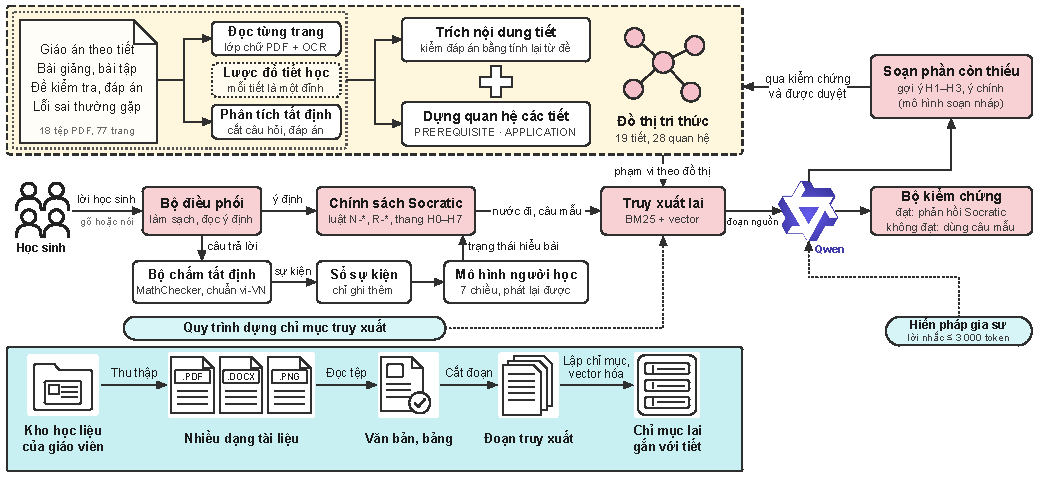
\includegraphics[width=1.1\linewidth]{figures/fig-architecture.pdf}}
\caption{Kiến trúc tổng thể của CAVAT, lấy từ bài báo. Sơ đồ vẽ khi Qwen còn là mô hình duy nhất viết lời; ở bản hiện hành hộp Qwen được thay bằng chuỗi nhiều mô hình do cổng AI điều phối, và Hình~\ref{fig:bandit-flow} bổ sung bộ chọn nước đi bằng bandit vào hộp chính sách Socratic.}
\label{fig:architecture}
\end{figure}

Khối dựng gói giáo án biến tài liệu của giáo viên thành nội dung có cấu trúc mà gia sư dạy được. Hệ thống đọc từng trang của tệp PDF bằng lớp chữ và nhận dạng ký tự, rồi tách thành ba luồng song song: lược đồ tiết học mà mỗi tiết là một đỉnh, phân tích tất định cắt câu hỏi và đáp án, và trích nội dung của từng tiết kèm kiểm đáp án bằng cách tính lại từ đề. Các quan hệ giữa tiết, gồm quan hệ tiên quyết và quan hệ vận dụng, được dựng thành đồ thị tri thức gồm $19$ tiết và $28$ quan hệ. Phần còn thiếu của tài liệu, chẳng hạn gợi ý ở các bậc từ H1 đến H3 hay các ý chính của bài, do mô hình ngôn ngữ soạn nháp, và bản nháp chỉ được dùng sau khi qua kiểm chứng và được giáo viên duyệt.

Khối hội thoại xử lý từng lượt nói của học sinh theo một chuỗi cố định. Bộ điều phối làm sạch lời học sinh và đọc ý định, chính sách Socratic chọn nước đi và mức gợi ý theo luật trên đồ thị và trên từng câu hỏi, và truy xuất lai tìm đoạn nguồn trong phạm vi mà đồ thị cho phép. Mô hình ngôn ngữ nhận nước đi, câu mẫu và đoạn nguồn trong một lời nhắc không quá $3\,000$ token, rồi viết lời gia sư. Bộ kiểm chứng kiểm lời đó: lời đạt thì được gửi cho học sinh, lời không đạt thì được thay bằng câu mẫu đã duyệt.

Khối chấm điểm tách biệt hoàn toàn với mô hình ngôn ngữ. Bộ chấm tất định theo chuẩn viết số của Việt Nam quyết định đúng sai của câu trả lời, mỗi kết quả được ghi thành một sự kiện vào sổ sự kiện chỉ ghi thêm, và mô hình người học bảy chiều tính lại mức hiểu bài từ sổ đó. Trạng thái hiểu bài quay lại làm đầu vào của chính sách để chọn nước đi cho lượt sau. Quy trình dựng chỉ mục ở dưới cùng thu thập kho học liệu của giáo viên gồm nhiều định dạng như PDF, DOCX và ảnh, đọc thành văn bản và bảng, cắt thành đoạn truy xuất, rồi lập chỉ mục và vector hóa để gắn mỗi đoạn với một tiết. Các mục sau của chương mô tả từng thành phần này chi tiết hơn.

\section{Yêu cầu phi chức năng}\label{sec:nfr}

\emph{(Đang biên soạn.)}

\section{Bộ chọn nước đi bằng contextual bandit}\label{sec:bandit-design}

\subsection{Vị trí trong hệ thống}
Bộ chọn bandit thay thế bộ chọn do mô hình ngôn ngữ làm ở mỗi lượt có nhiều nước đi hợp lệ. Chính sách dạy vẫn là bên đưa ra tập nước đi: ở mỗi lượt, chính sách trả về tối đa ba nước đi, nước đứng đầu là nước của chính sách, và không nước nào giúp nhiều hơn nước đó. Bộ chọn chỉ chọn một nước trong tập này, và chính sách kiểm lại lựa chọn trước khi chơi. Bandit vì vậy không thể chọn nước ngoài thực đơn, không chọn trong lượt kiểm tra cuối tiết, và không đụng tới các luật cố định như giới hạn thời gian, giải thích đầy đủ hay trần gợi ý của câu kiểm tra. Hình~\ref{fig:bandit-flow} mô tả vòng chọn và vòng học.

\begin{figure}[ht]
\centering
\begin{tikzpicture}[font=\footnotesize,
  box/.style={draw=black,line width=0.5pt,fill=white,align=center,minimum height=13mm,text width=29mm,inner sep=2pt},
  bnd/.style={box,fill=gray!30,dashed,line width=0.7pt},
  store/.style={box,fill=gray!14},
  arr/.style={-{Stealth[length=2mm,width=1.6mm]},line width=0.6pt},
  lab/.style={font=\scriptsize\itshape,fill=white,inner sep=1pt}]
\node[box] (menu) at (0,0) {\textbf{Chính sách}\\\scriptsize thực đơn tối đa ba nước đi};
\node[bnd] (bandit) at (4.2,0) {\textbf{Bandit}\\\scriptsize ngữ cảnh $x$, điểm UCB, $\varepsilon$-tham lam};
\node[box] (accept) at (8.4,0) {\textbf{Chính sách kiểm lại}\\\scriptsize chỉ chơi nước trong thực đơn};
\node[box] (play) at (12.6,0) {\textbf{Nước đi được chơi}\\\scriptsize ghi \texttt{MOVE\_CHOSEN}};
\node[box] (ans) at (12.6,-3.0) {\textbf{Câu trả lời có chấm kế tiếp}\\\scriptsize đúng, một phần, sai};
\node[box] (rew) at (8.4,-3.0) {\textbf{Sự kiện}\\\scriptsize \texttt{BANDIT\_REWARD}};
\node[store] (arms) at (4.2,-3.0) {\textbf{Kho \texttt{bandit\_arms}}\\\scriptsize $\sum xx^{\top}$, $\sum rx$, $n$};
\draw[arr] (menu) -- node[lab,above]{các nước} (bandit);
\draw[arr] (bandit) -- node[lab,above]{một nước} (accept);
\draw[arr] (accept) -- (play);
\draw[arr] (play) -- node[lab,right]{con trả lời} (ans);
\draw[arr] (ans) -- node[lab,above]{thưởng} (rew);
\draw[arr] (rew) -- node[lab,above]{$\$inc$} (arms);
\draw[arr] (arms) -- node[lab,right]{trạng thái} (bandit);
\end{tikzpicture}

\caption{Vòng chọn và vòng học của bộ chọn bandit. Hàng trên là lượt chọn, hàng dưới là cách câu trả lời kế tiếp của học sinh trở thành phần thưởng và cập nhật kho trạng thái.}
\label{fig:bandit-flow}
\end{figure}

\subsection{Cánh tay, ngữ cảnh và phần thưởng}
Cánh tay là loại nước đi cùng bậc của nó, chẳng hạn hỏi lại cách làm, gợi ý ở bậc hai hay đưa phản ví dụ. Cách định nghĩa này làm cùng một cánh tay mang cùng một nghĩa trên mọi thực đơn, dù thực đơn gồm những nước nào. Các nước đóng câu hoặc xác nhận để sang câu sau không phải cánh tay của bandit. Thực đơn có nước như vậy, chẳng hạn lượt hỏi ``vì sao'' sau một câu đúng, được bộ chọn chuyển cho bộ chọn dự phòng hoặc giữ nước của chính sách.

Ngữ cảnh là chín số trong đoạn $[0,1]$ rút từ tình hình của học sinh trên câu đang làm, mô tả ở Bảng~\ref{tab:bandit-context}. Ngữ cảnh chỉ gồm số đếm và không chứa lời của học sinh hay đáp án của câu hỏi, nên bandit không thể làm lộ đáp án.

\begin{table}[ht]
\centering
\caption{Chín thành phần của vector ngữ cảnh và cách chuẩn hóa về đoạn $[0,1]$.}
\label{tab:bandit-context}
\small
\begin{tabularx}{\linewidth}{@{}lXr@{}}
\toprule
Thành phần & Ý nghĩa & Chuẩn hóa \\
\midrule
Hệ số tự do & Hằng số $1$ cho phần tử chặn & $1$ \\
Số lần trả lời & Số lần học sinh đã trả lời câu này & $\min(n,5)/5$ \\
Số gợi ý & Số gợi ý học sinh đã nhận & $\min(n,4)/4$ \\
Bậc gợi ý cao nhất & Bậc cao nhất đã dùng trên thang H0--H7 & $h/7$ \\
Lượt chưa tiến bộ & Số lượt không tiến bộ liên tiếp & $\min(n,4)/4$ \\
Lần xin gợi ý & Số lần học sinh chủ động xin gợi ý & $\min(n,3)/3$ \\
Dấu hiệu nản & Số lần học sinh nói ra sự nản chí & $\min(n,3)/3$ \\
Đã hỏi cách làm & Gia sư đã hỏi ``con làm thế nào'' chưa & $0$ hoặc $1$ \\
Lỗi lặp lại nhiều nhất & Số lần lặp lại của lỗi quan niệm thường gặp nhất & $\min(n,3)/3$ \\
\bottomrule
\end{tabularx}
\end{table}

Phần thưởng của một lượt chọn là giá trị của câu trả lời có chấm kế tiếp của học sinh trên cùng câu, trừ chi phí theo mức giúp của nước đi. Câu trả lời đúng được $1$, đúng một phần được $0{,}5$ và sai được $0$. Chi phí bằng $0{,}3$ nhân mức giúp của nước đi chia cho $7$, với mức giúp lấy từ bậc trên thang gợi ý và bằng $0$ cho nước hỏi lại. Một gợi ý bậc nhất đưa học sinh tới câu đúng vì thế được $1-0{,}3/7\approx 0{,}96$, còn một câu hỏi lại đưa học sinh tới câu đúng được đúng $1$. Cách tính này khiến bandit ưa nước giúp ít mà vẫn có tác dụng, phù hợp với nguyên tắc Socratic ở Mục~\ref{sec:socratic-ref}. Lượt chọn mà học sinh không có câu trả lời có chấm nào theo sau, vì câu đóng trước, không được trả thưởng, và lượt chọn bị chính sách từ chối cũng không được trả thưởng.

\subsection{Quy tắc chọn và nhật ký}
Mỗi cánh tay trong thực đơn nhận điểm cận trên tin cậy của LinUCB theo công thức~\eqref{eq:linucb} với $\alpha=0{,}5$ và ridge bằng $1$. Bộ chọn lấy cánh tay có điểm cao nhất với xác suất $0{,}9$ và chọn ngẫu nhiên đều trong thực đơn với xác suất $0{,}1$. Hai cánh tay hòa điểm thì cánh tay đứng đầu thực đơn thắng, tức nước của chính sách. Hệ quả là một bandit chưa học gì chơi đúng nước mà chính sách sẽ chơi. Số ngẫu nhiên sinh từ mã băm của khóa phiên, số lượt và đề bài, nên cùng phiên, cùng lượt và cùng thực đơn luôn cho cùng một lựa chọn.

Mỗi lượt chọn của bandit được ghi vào nhật ký sự kiện cùng cánh tay, xác suất của lượt chọn, vector ngữ cảnh và điểm của mọi cánh tay trong thực đơn. Sự kiện phần thưởng ghi cánh tay, ngữ cảnh, phần thưởng và phiên bản của bandit. Buổi học dựng lại từ nhật ký đọc lượt chọn đã ghi thay vì hỏi bandit lại, và dựng lại mà vẫn nhớ lượt chọn nào đang chờ phần thưởng, nên không lượt chọn nào bị trả thưởng hai lần.

\subsection{Trạng thái học và lưu trữ}
Trạng thái của bandit gồm ba đại lượng cộng được cho mỗi cánh tay: tổng $\sum xx^{\top}$, tổng $\sum rx$ và số lượt. Tính cộng được có hai hệ quả. Hệ quả đầu là thứ tự các phần thưởng không ảnh hưởng tới trạng thái, giống tính giao hoán của cập nhật Beta--Bernoulli. Hệ quả sau là mỗi phần thưởng là một phép cộng nguyên tử vào một document duy nhất, phù hợp với cơ sở dữ liệu không có giao dịch trên nhiều document. Mỗi document thuộc một trường, một phiên bản bandit và một cánh tay, và mọi truy vấn bắt buộc lọc theo trường. Cập nhật diễn ra sau khi lệnh của học sinh được ghi thành công, nên lệnh lặp không làm trả thưởng hai lần. Toàn bộ kho là một phép chiếu của các sự kiện phần thưởng và dựng lại được khi cần. Không mô hình ngôn ngữ nào ghi vào kho này.

\subsection{Cách bật và các bất biến được giữ}
Tham số cấu hình \texttt{TUTOR\_CHOOSER=bandit} bật bộ chọn bandit, còn mặc định vẫn là bộ chọn do mô hình ngôn ngữ làm cho tới khi chủ dự án duyệt các tham số của bandit. Bandit giữ nguyên cả sáu bất biến của đồ án: chính sách quyết định nước đi và kiểm lại lựa chọn, đáp án không đi vào bandit, bộ chấm vẫn tất định, trạng thái học là phép gập của sự kiện, dữ liệu gắn định danh trường, và mô hình ngôn ngữ không ghi mức hiểu bài.

\newpage\cleardoublepage
\chapter{Triển khai, thực nghiệm và đánh giá}\label{chap:eval}
Chương này trình bày việc triển khai hệ thống, phương pháp đánh giá và kết quả thực nghiệm theo năm câu hỏi nghiên cứu.

\section{Phương pháp đánh giá}\label{sec:eval-method}
\emph{(Đang biên soạn.)}

\section{Kết quả truy xuất}\label{sec:eval-rag}
\emph{(Đang biên soạn.)}

\section{Hành vi Socratic và so sánh với thị trường}\label{sec:eval-socratic}
\emph{(Đang biên soạn.)}

\section{Chấm câu trả lời của trẻ}\label{sec:eval-grading}
\emph{(Đang biên soạn.)}

\section{Mô hình người học}\label{sec:eval-learner}
\emph{(Đang biên soạn.)}

\section{Bộ chọn nước đi bằng bandit}\label{sec:eval-bandit}

\subsection{Môi trường mô phỏng}
Câu hỏi thứ năm (RQ5) hỏi bộ chọn bandit học được lựa chọn phụ thuộc ngữ cảnh nhanh đến đâu và log của nó có đủ để đánh giá một chính sách khác hay không. Việc trả lời cần một môi trường trong đó nước đi tốt nhất thay đổi theo học sinh, nên đồ án dựng một môi trường mô phỏng khai báo thay vì dùng dữ liệu của trẻ thật, vì chưa có đủ dữ liệu thật để huấn luyện hay đánh giá. Môi trường sinh ở mỗi lượt tình hình của học sinh với chín thành phần của vector ngữ cảnh, sinh một trong ba loại thực đơn mà chính sách có thể đưa ra, rồi quyết định học sinh trả lời đúng hay sai ở câu kế tiếp. Xác suất trả lời đúng là hàm logistic của ngữ cảnh với một vector trọng số riêng cho mỗi nước đi. Nước hỏi lại cách làm có xác suất cao với học sinh đang tự suy nghĩ và thấp với học sinh bế tắc, còn các gợi ý ở bậc cao có xu hướng ngược lại. Nước tốt nhất là hỏi lại cách làm ở $44\%$ ngữ cảnh, gợi ý bậc một ở $38\%$ và gợi ý bậc hai ở $18\%$, nên bandit có điều để học.

Môi trường này là một khai báo của đồ án, không phải số đo trên học sinh. Kết quả vì vậy cho biết thuật toán có học được lựa chọn phụ thuộc ngữ cảnh hay không và học nhanh ra sao, không cho biết nước đi nào giúp học sinh thật. Chính sách của hệ thống không có cách nào làm tốt hơn trên môi trường này vì nó không đọc ngữ cảnh, nên khoảng cách giữa chính sách và bandit ở bảng dưới phản ánh cách khai báo môi trường chứ không phản ánh dữ liệu thật.

\subsection{Các chính sách so sánh}
Năm chính sách được so sánh. Chính sách thứ nhất là nước mặc định của chính sách dạy, tức nước đứng đầu thực đơn, là hành vi của hệ thống khi không có bộ chọn nào. Chính sách ngẫu nhiên chọn đều trong thực đơn. Chính sách giúp ít nhất luôn chọn nước giúp ít nhất, một quy tắc thủ công hợp lý theo nguyên tắc Socratic. Hai biến thể của bandit gồm bản đang cấu hình ($\alpha=0{,}5$, $\varepsilon=0{,}1$) và bản không thăm dò ngẫu nhiên ($\varepsilon=0$). Oracle biết xác suất thật và chọn nước tốt nhất, cho cận trên.

\subsection{Kết quả}
Mỗi chính sách chạy $3\,000$ lượt trên $30$ hạt giống ngẫu nhiên, và Bảng~\ref{tab:bandit-results} báo trung bình cùng khoảng tin cậy $95\%$ của hối tiếc tích lũy, tỉ lệ chọn đúng nước tốt nhất và phần thưởng trung bình ở một phần tư số lượt cuối.

% Sinh bởi tools/bandit_tex.py từ docs/thesis/data/bandit-eval.json; không sửa tay.
\begin{table}[ht]
\centering
\caption{Kết quả trên môi trường mô phỏng, $3\,000$ lượt, $30$ hạt giống, trung bình $\pm$ khoảng tin cậy $95\%$. Hai cột cuối tính trên một phần tư số lượt cuối.}
\label{tab:bandit-results}
\small
\begin{tabularx}{\linewidth}{@{}Xrrr@{}}
\toprule
Chính sách & Hối tiếc tích lũy & Chọn đúng nước tốt nhất & Phần thưởng \\
\midrule
Nước của chính sách & $878{,}9 \pm 5{,}8$ & $0{,}315 \pm 0{,}005$ & $0{,}488 \pm 0{,}007$ \\
Ngẫu nhiên & $621{,}1 \pm 5{,}6$ & $0{,}389 \pm 0{,}005$ & $0{,}573 \pm 0{,}006$ \\
Giúp ít nhất & $368{,}6 \pm 5{,}0$ & $0{,}693 \pm 0{,}006$ & $0{,}657 \pm 0{,}006$ \\
Bandit ($\varepsilon=0{,}1$) & $93{,}5 \pm 3{,}0$ & $0{,}833 \pm 0{,}009$ & $0{,}759 \pm 0{,}004$ \\
Bandit ($\varepsilon=0$) & $73{,}9 \pm 41{,}0$ & $0{,}841 \pm 0{,}046$ & $0{,}763 \pm 0{,}015$ \\
Oracle & $0{,}0 \pm 0{,}0$ & $1{,}000 \pm 0{,}000$ & $0{,}783 \pm 0{,}004$ \\
\bottomrule
\end{tabularx}
\end{table}


Bandit giảm hối tiếc tích lũy từ $878{,}9$ của nước mặc định xuống $93{,}5$, tức xuống dưới $11\%$, và còn khoảng một phần tư hối tiếc của quy tắc giúp ít nhất. Bandit chọn đúng nước tốt nhất ở $83{,}3\%$ số lượt trong một phần tư cuối và đạt phần thưởng $0{,}759$ so với $0{,}783$ của oracle. Hình~\ref{fig:bandit-regret} cho thấy hối tiếc trung bình mỗi lượt của bandit giảm nhanh trong vài trăm lượt đầu rồi ổn định ở mức thấp, trong khi các chính sách cố định giữ nguyên mức hối tiếc của mình.

\begin{figure}[ht]
\centering
% Sinh bởi tools/bandit_tex.py từ docs/thesis/data/bandit-eval.json; không sửa tay.
\begin{tikzpicture}
\begin{axis}[width=0.92\linewidth,height=6.4cm,xlabel={số lượt đã chơi},ylabel={hối tiếc trung bình mỗi lượt},xmin=0,xmax=3000,ymin=0,ymajorgrids,xtick={0,1000,2000,3000},
  legend style={font=\footnotesize,at={(0.5,-0.32)},anchor=north,legend columns=3,draw=none},
  tick label style={font=\footnotesize},label style={font=\small},axis lines=left]
\addplot[black,dotted,line width=0.9pt] coordinates {(100,0.2943) (200,0.2928) (300,0.2955) (400,0.2880) (500,0.2951) (600,0.2936) (700,0.2894) (800,0.2860) (900,0.2941) (1000,0.2903) (1100,0.2967) (1200,0.2849) (1300,0.2927) (1400,0.2879) (1500,0.2943) (1600,0.2866) (1700,0.2977) (1800,0.2937) (1900,0.2961) (2000,0.2963) (2100,0.3024) (2200,0.2913) (2300,0.2904) (2400,0.2976) (2500,0.2884) (2600,0.2913) (2700,0.2962) (2800,0.2956) (2900,0.2890) (3000,0.3010)};
\addplot[black!60,dashed,line width=0.9pt] coordinates {(100,0.2059) (200,0.2084) (300,0.2063) (400,0.2158) (500,0.2069) (600,0.2094) (700,0.2036) (800,0.2018) (900,0.2047) (1000,0.2006) (1100,0.2055) (1200,0.2072) (1300,0.2060) (1400,0.2114) (1500,0.2052) (1600,0.1988) (1700,0.2031) (1800,0.2052) (1900,0.2077) (2000,0.2109) (2100,0.2117) (2200,0.2099) (2300,0.2045) (2400,0.2080) (2500,0.2047) (2600,0.2128) (2700,0.2118) (2800,0.2080) (2900,0.2026) (3000,0.2126)};
\addplot[black!60,dash dot,line width=0.9pt] coordinates {(100,0.1203) (200,0.1182) (300,0.1295) (400,0.1192) (500,0.1246) (600,0.1262) (700,0.1301) (800,0.1205) (900,0.1244) (1000,0.1070) (1100,0.1231) (1200,0.1271) (1300,0.1234) (1400,0.1175) (1500,0.1203) (1600,0.1238) (1700,0.1212) (1800,0.1330) (1900,0.1208) (2000,0.1204) (2100,0.1190) (2200,0.1235) (2300,0.1283) (2400,0.1266) (2500,0.1162) (2600,0.1216) (2700,0.1271) (2800,0.1243) (2900,0.1242) (3000,0.1247)};
\addplot[black,solid,line width=1.2pt] coordinates {(100,0.1091) (200,0.0543) (300,0.0410) (400,0.0378) (500,0.0310) (600,0.0304) (700,0.0291) (800,0.0282) (900,0.0288) (1000,0.0303) (1100,0.0285) (1200,0.0255) (1300,0.0250) (1400,0.0256) (1500,0.0267) (1600,0.0215) (1700,0.0264) (1800,0.0255) (1900,0.0286) (2000,0.0290) (2100,0.0236) (2200,0.0279) (2300,0.0265) (2400,0.0237) (2500,0.0250) (2600,0.0226) (2700,0.0295) (2800,0.0224) (2900,0.0252) (3000,0.0265)};
\addplot[black!45,solid,line width=0.9pt] coordinates {(100,0.0968) (200,0.0378) (300,0.0300) (400,0.0283) (500,0.0280) (600,0.0250) (700,0.0269) (800,0.0224) (900,0.0258) (1000,0.0239) (1100,0.0213) (1200,0.0214) (1300,0.0210) (1400,0.0210) (1500,0.0203) (1600,0.0204) (1700,0.0190) (1800,0.0185) (1900,0.0184) (2000,0.0184) (2100,0.0188) (2200,0.0194) (2300,0.0208) (2400,0.0181) (2500,0.0195) (2600,0.0194) (2700,0.0182) (2800,0.0199) (2900,0.0200) (3000,0.0203)};
\legend{{Nước của chính sách},{Ngẫu nhiên},{Giúp ít nhất},{Bandit ($\varepsilon=0{,}1$)},{Bandit ($\varepsilon=0$)}}
\end{axis}
\end{tikzpicture}

\caption{Hối tiếc trung bình mỗi lượt, tính theo khối $100$ lượt và trung bình trên $30$ hạt giống. Các chính sách cố định không học nên giữ nguyên mức hối tiếc.}
\label{fig:bandit-regret}
\end{figure}

Bản bandit không thăm dò có hối tiếc trung bình thấp hơn nhưng khoảng tin cậy rộng hơn mười lần ($73{,}9\pm41{,}0$ so với $93{,}5\pm3{,}0$). Một số hạt giống của bản này kẹt ở một cánh tay xấu vì thuật toán không bao giờ thử lại cánh tay khác khi các cánh tay đều có điểm gần nhau. Thăm dò ngẫu nhiên $\varepsilon=0{,}1$ giữ độ rộng này ở mức nhỏ, và đồng thời cho xác suất dương cho mọi lượt chọn, điều kiện cần của đánh giá ngoài chính sách ở mục sau.

\subsection{Đánh giá ngoài chính sách từ nhật ký}
Một bandit với $\varepsilon=0{,}3$ chạy $3\,000$ lượt trên mỗi hạt giống và ghi xác suất của từng lượt chọn. Công thức~\eqref{eq:ips} ước lượng từ nhật ký đó giá trị của hai chính sách đích tất định chưa từng chạy, gồm chính sách giúp ít nhất và oracle. Ước lượng cho chính sách giúp ít nhất là $0{,}665\pm0{,}007$ so với giá trị thật $0{,}661$, và cho oracle là $0{,}788\pm0{,}006$ so với $0{,}782$. Sai lệch nằm trong khoảng tin cậy của ước lượng, nên nhật ký của bandit đủ để so sánh các chính sách đích mà không cần chạy chúng trên học sinh. Đây là lý do đồ án ghi xác suất của mỗi lượt chọn vào nhật ký sự kiện.

\subsection{Thảo luận và giới hạn}
Kết quả chứng minh được rằng bộ chọn bandit học một lựa chọn phụ thuộc ngữ cảnh trong vài trăm lượt, không bao giờ chọn nước ngoài thực đơn của chính sách và để lại nhật ký đủ dùng cho đánh giá ngoài chính sách. Kết quả không chứng minh bandit giúp học sinh thật học tốt hơn, vì môi trường là khai báo. Phần thưởng chỉ nhìn một câu trả lời kế tiếp, nên bandit có thể ưa nước làm học sinh đúng ngay hơn nước giúp học sinh hiểu sâu. Hệ số chi phí của sự giúp đỡ và các tham số của thuật toán chưa được chủ dự án duyệt, và bộ chọn bandit chưa chạy trên buổi học thật nên chưa là cấu hình mặc định. Bandit gộp dữ liệu của cả trường chứ chưa tách theo từng học sinh, và các cánh tay hiếm xuất hiện trong thực đơn học chậm hơn các cánh tay phổ biến.

\newpage\cleardoublepage
\chapter{Kết luận}\label{chap:conclusion}
Chương này tổng kết kết quả đạt được, nêu các hạn chế và hướng phát triển.

\section{Những công việc đã thực hiện trong đồ án}

\emph{(Đang biên soạn.)}

\newpage\cleardoublepage

\nocite{*}
\phantomsection 
\addcontentsline{toc}{chapter}{Tài liệu tham khảo}
\bibliography{references}\newpage\cleardoublepage
\end{document}